\chapter{Dữ liệu Công cụ Tìm kiếm}
\label{ch:M4L2}

% Lesson: Search Engine Data

\section*{Lesson Notes}

MODULE 4 | BÀI 2

{\small
\begin{longtable}{>{\raggedright\arraybackslash}p{0.213\linewidth}>{\raggedright\arraybackslash}p{0.727\linewidth}}
\toprule
\textbf{Thời gian đọc} & 60 phút \\
\addlinespace[2pt]
\textbf{Kiến thức nền tảng} & Python cơ bản, các khái niệm cơ bản về Xử lý ngôn ngữ tự nhiên, thị trường tài chính \\
\addlinespace[2pt]
\textbf{Từ khóa} & Học máy, Google Trends, Pytrends, phân tích cảm xúc, TF-IDF, LSA (Phân tích Ngữ nghĩa Tiềm ẩn), NLP (Xử lý ngôn ngữ tự nhiên) \\
\addlinespace[2pt]
\bottomrule
\end{longtable}
}

\emph{Trong bài học này, chúng ta khám phá cách tận dụng khoa học dữ liệu và học máy cho phân tích tài chính, với trọng tâm là phân tích các từ khóa tìm kiếm từ dữ liệu Google Trends. Bài học đề cập các kỹ thuật như TF-IDF và LSA để trích xuất thông tin từ văn bản, đồng thời minh họa cách thu thập và phân tích dữ liệu Google Trends bằng Python và thư viện \texttt{pytrends}. Notebook cũng thảo luận việc ứng dụng các kỹ thuật này cho phân tích cảm xúc, quản trị rủi ro và tối ưu hóa danh mục đầu tư.}

\begin{lstlisting}[language=Python,escapeinside={(*@}{@*)}]
# (*@Tải@*) (*@các@*) (*@thư@*) (*@viện@*)
import matplotlib.pyplot as plt
import nltk
import pandas as pd
import plotly.graph_objects as go
import re
import time
import pytrends

from nltk.corpus import stopwords
from nltk.stem import WordNetLemmatizer
from pytrends.request import TrendReq
from sklearn.decomposition import TruncatedSVD
from sklearn.feature_extraction.text import CountVectorizer, TfidfVectorizer
from sklearn.metrics.pairwise import cosine_similarity

# (*@Tải@*) (*@tài@*) (*@nguyên@*) (*@'punkt'@*)
nltk.download('punkt')
nltk.download('punkt_tab')
\end{lstlisting}

\begin{lstlisting}[escapeinside={(*@}{@*)}]
[nltk_data] Downloading package punkt to /root/nltk_data...
[nltk_data]   Unzipping tokenizers/punkt.zip.
[nltk_data] Downloading package punkt_tab to /root/nltk_data...
[nltk_data]   Unzipping tokenizers/punkt_tab.zip.
\end{lstlisting}

\begin{lstlisting}[escapeinside={(*@}{@*)}]
True
\end{lstlisting}

\section*{1. Dữ liệu Công cụ Tìm kiếm là gì}

Dữ liệu công cụ tìm kiếm là thông tin được thu thập và tạo ra bởi các công cụ tìm kiếm khi người dùng tương tác với chúng. Dữ liệu này bao gồm nhiều khía cạnh của hành vi người dùng, sở thích và các tương tác trong hệ sinh thái công cụ tìm kiếm. Dữ liệu công cụ tìm kiếm là một nguồn dữ liệu thay thế có giá trị, có thể bổ sung cho dữ liệu tài chính truyền thống và mang lại một góc nhìn độc đáo về xu hướng thị trường và hành vi của nhà đầu tư.

Trong lĩnh vực kỹ thuật tài chính, việc sử dụng dữ liệu công cụ tìm kiếm là một mảng chuyên biệt hơn. Nhìn chung chúng ta có hai lựa chọn: sử dụng API từ các công cụ tìm kiếm lớn như Google Trends API hoặc Bing API; hoặc sử dụng các nhà cung cấp dữ liệu thay thế: một số công ty chuyên cung cấp dữ liệu thay thế cho phân tích tài chính, bao gồm cả dữ liệu công cụ tìm kiếm.

Trong bài học này, chúng ta sẽ tập trung vào dữ liệu Google Trends. Dưới đây là một số gợi ý về cách dữ liệu Google Trends có thể được sử dụng cho các tác vụ kỹ thuật tài chính:

\begin{itemize}
  \item \textbf{Phân tích cảm xúc:} Dữ liệu Google Trends có thể được dùng để đo lường cảm xúc của thị trường đối với một chứng khoán hoặc tài sản cụ thể. Điều này có thể thực hiện bằng cách theo dõi khối lượng tìm kiếm của các từ khóa liên quan đến chứng khoán hoặc tài sản đó. Ví dụ, nếu khối lượng tìm kiếm cho ``Tesla stock price'' đang tăng, đây có thể là dấu hiệu cho thấy thị trường đang trở nên lạc quan hơn về Tesla.
  \item \textbf{Mô hình dự báo:} Dữ liệu Google Trends có thể được dùng để xây dựng các mô hình dự báo cho thị trường tài chính. Điều này có thể thực hiện bằng cách dùng các thuật toán học máy để huấn luyện mô hình trên dữ liệu Google Trends lịch sử và các nguồn dữ liệu liên quan khác. Ví dụ, một mô hình có thể được huấn luyện để dự báo giá của một cổ phiếu dựa trên khối lượng tìm kiếm của các từ khóa liên quan đến cổ phiếu đó.
  \item \textbf{Quản trị rủi ro:} Dữ liệu Google Trends có thể được dùng để nhận diện và quản lý rủi ro trên thị trường tài chính. Điều này có thể thực hiện bằng cách theo dõi khối lượng tìm kiếm của các từ khóa liên quan đến các yếu tố rủi ro, chẳng hạn ``economic recession'' hoặc ``market volatility''. Ví dụ, nếu khối lượng tìm kiếm cho ``economic recession'' đang tăng, đây có thể là dấu hiệu cho thấy thị trường ngày càng lo ngại về khả năng xảy ra suy thoái.
  \item \textbf{Giao dịch thuật toán:} Dữ liệu Google Trends có thể được dùng để phát triển các chiến lược giao dịch thuật toán. Điều này có thể thực hiện bằng cách dùng dữ liệu Google Trends để xác định các cơ hội giao dịch. Ví dụ, một chiến lược giao dịch có thể được phát triển để mua một cổ phiếu khi khối lượng tìm kiếm của các từ khóa liên quan đến cổ phiếu đó đang tăng.
\end{itemize}

Dữ liệu công cụ tìm kiếm có thể có giá trị đối với nhà đầu tư, và TF-IDF có thể đóng vai trò trong việc phân tích nó. Cụ thể như sau:

\textbf{Dữ liệu công cụ tìm kiếm giúp ích cho nhà đầu tư như thế nào:}

\begin{itemize}
  \item Đánh giá mức độ quan tâm của công chúng: Dữ liệu công cụ tìm kiếm, như Google Trends, cho thấy mức độ phổ biến tương đối của các từ khóa tìm kiếm theo thời gian. Điều này có thể phản ánh mức độ quan tâm của công chúng đối với các công ty, sản phẩm, ngành hoặc xu hướng kinh tế cụ thể.
  \item Nhận diện các xu hướng mới nổi: Khối lượng tìm kiếm tăng lên đối với các từ khóa cụ thể có thể báo hiệu các xu hướng mới nổi hoặc những thay đổi trong hành vi người tiêu dùng, mang lại các cơ hội đầu tư sớm.
  \item Phân tích cảm xúc: Phân tích các truy vấn tìm kiếm liên quan đến một công ty hoặc tài sản có thể cung cấp hiểu biết về cảm xúc của công chúng, vốn có thể ảnh hưởng đến các quyết định đầu tư.
  \item Mô hình dự báo: Dữ liệu công cụ tìm kiếm có thể được kết hợp với các nguồn dữ liệu khác để xây dựng các mô hình dự báo diễn biến thị trường hoặc hiệu quả hoạt động của công ty.
\end{itemize}

\textbf{Vai trò của TF-IDF trong phân tích dữ liệu công cụ tìm kiếm:}

\begin{itemize}
  \item Phân tích từ khóa: TF-IDF có thể được áp dụng để phân tích chính các truy vấn tìm kiếm, xác định những thuật ngữ liên quan và giàu thông tin nhất đối với một chủ đề đầu tư.
  \item Phân tích tài liệu: TF-IDF có thể được dùng để phân tích nội dung của các trang web trả về trong kết quả tìm kiếm, giúp nhà đầu tư hiểu bối cảnh và cảm xúc xoay quanh một từ khóa tìm kiếm cụ thể.
  \item Nhận diện xu hướng: Theo dõi sự thay đổi điểm TF-IDF của các thuật ngữ cụ thể theo thời gian có thể giúp nhận diện các xu hướng mới nổi hoặc sự thay đổi trong mức độ quan tâm của công chúng.
  \item Ví dụ:
  \begin{itemize}
    \item Một nhà đầu tư có thể phân tích dữ liệu Google Trends cho các từ khóa liên quan đến xe điện để đánh giá mức độ quan tâm ngày càng tăng đối với ngành này và nhận diện các cơ hội đầu tư tiềm năng.
    \item Một quỹ phòng hộ có thể dùng TF-IDF để phân tích các bài báo và bài đăng trên mạng xã hội liên quan đến một công ty nhằm đánh giá cảm xúc của công chúng và dự báo các biến động giá cổ phiếu có thể xảy ra.
  \end{itemize}
\end{itemize}

\textbf{Lợi ích đối với nhà đầu tư:}

\begin{itemize}
  \item Tín hiệu sớm: Dữ liệu công cụ tìm kiếm có thể cung cấp các tín hiệu sớm về xu hướng thị trường hoặc những thay đổi trong cảm xúc của nhà đầu tư.
  \item Nguồn dữ liệu thay thế: Nó cung cấp một nguồn dữ liệu thay thế có thể bổ sung cho dữ liệu tài chính truyền thống.
  \item Cải thiện việc ra quyết định: Bằng cách đưa phân tích dữ liệu công cụ tìm kiếm vào quy trình, nhà đầu tư có thể đưa ra các quyết định đầu tư sáng suốt hơn.
\end{itemize}

\textbf{Các lưu ý:}

\begin{itemize}
  \item Chất lượng dữ liệu: Dữ liệu công cụ tìm kiếm có thể nhiễu và không phải lúc nào cũng phản ánh chính xác cảm xúc thị trường.
  \item Mối quan ngại về quyền riêng tư: Cần tính đến các cân nhắc về đạo đức và các quy định về quyền riêng tư dữ liệu khi sử dụng dữ liệu công cụ tìm kiếm.
\end{itemize}

Nhìn chung, dữ liệu công cụ tìm kiếm có thể là một công cụ có giá trị đối với nhà đầu tư, và TF-IDF có thể được sử dụng hiệu quả để phân tích dữ liệu này và trích xuất những hiểu biết có ý nghĩa phục vụ các quyết định đầu tư.

\subsection*{1.1 Giới thiệu về dữ liệu Google Trends}

Cần lưu ý rằng dữ liệu Google Trends chỉ là một trong nhiều nguồn dữ liệu có thể được sử dụng cho các tác vụ kỹ thuật tài chính. Việc sử dụng nhiều nguồn dữ liệu khác nhau là quan trọng để có bức tranh đầy đủ về thị trường.

Trong bài học này, chúng ta sẽ khám phá cách dùng Python để tải và phân tích dữ liệu từ Google Trends, một công cụ mạnh mẽ cho biết tần suất một từ khóa tìm kiếm cụ thể được nhập vào, so với tổng khối lượng tìm kiếm trên nhiều khu vực khác nhau của thế giới và bằng nhiều ngôn ngữ khác nhau. Chúng ta sẽ dùng thư viện \texttt{pytrends}, một giao diện Python cho dữ liệu Google Trends. Thư viện này cho phép tự động hóa việc tải xuống các báo cáo từ Google Trends. Chúng ta sẽ học cách lấy mức độ quan tâm theo thời gian (interest over time) cho một từ khóa tìm kiếm cụ thể, cách phân tích dữ liệu này bằng Python, và cách trực quan hóa các phát hiện. Thư viện cung cấp một giao diện tới Google Trends, cho phép:

\begin{itemize}
  \item Lấy mức độ quan tâm theo thời gian (Fetch Interest Over Time): Xem mức độ quan tâm tìm kiếm đối với các từ khóa cụ thể đã thay đổi như thế nào trong một khoảng thời gian.
  \item Phân tích mức độ quan tâm theo khu vực (Analyze Interest by Region): Khám phá nơi nào trên thế giới người ta tìm kiếm các từ khóa cụ thể.
  \item Tìm các truy vấn liên quan (Find Related Queries): Nhận diện các truy vấn tìm kiếm hàng đầu (top) và đang tăng (rising) liên quan đến các từ khóa của chúng ta.
\end{itemize}

Đến cuối phần này, chúng ta sẽ có hiểu biết vững chắc về cách tận dụng Python và dữ liệu Google Trends để khám phá các hiểu biết về xu hướng tìm kiếm. Kiến thức này có thể đặc biệt hữu ích trong các lĩnh vực như nghiên cứu thị trường, nơi việc hiểu các xu hướng có thể mang lại những hiểu biết giá trị về hành vi người tiêu dùng.

TooManyRequestsError: The request failed: Google returned a response with code 429

\subsection*{1.2 Lấy và So sánh Mức độ Quan tâm theo Thời gian}

Bây giờ hãy xác định các từ khóa tìm kiếm mà chúng ta muốn so sánh. Trong trường hợp này, chúng ta sẽ so sánh ``AAPL'', ``TSLA'' và ``NVDA''. Chúng ta lấy mức độ quan tâm trong khoảng 12 tháng gần nhất đối với các từ khóa tìm kiếm này từ Google Trends và trực quan hóa dữ liệu. Đoạn mã sau khởi tạo một đối tượng của lớp \texttt{TrendReq} từ thư viện \texttt{pytrends} và định nghĩa một danh sách từ khóa cùng một khung thời gian. Việc này thiết lập các đối tượng cần thiết để tương tác với Google Trends và truy xuất dữ liệu. Sau đó, đoạn mã xây dựng payload cho yêu cầu Google Trends bằng các từ khóa và khung thời gian đã định nghĩa, rồi truy xuất dữ liệu mức độ quan tâm theo thời gian. DataFrame \texttt{interest\_over\_time\_df} khi đó sẽ chứa dữ liệu Google Trends cho các từ khóa và khung thời gian đã chỉ định:

\begin{lstlisting}[language=Python,escapeinside={(*@}{@*)}]
# (*@Khởi@*) (*@tạo@*) (*@một@*) (*@đối@*) (*@tượng@*) (*@của@*) (*@lớp@*) (*@TrendReq@*) (*@với@*) (*@khu@*) (*@vực@*) (*@US@*) (*@và@*) (*@múi@*) (*@giờ@*) (*@360@*)
pytrends = TrendReq(hl='en-US', tz=360)

# (*@Định@*) (*@nghĩa@*) (*@danh@*) (*@sách@*) (*@từ@*) (*@khóa@*) (*@và@*) (*@khung@*) (*@thời@*) (*@gian@*)
kw_list = ["AAPL", "TSLA", "NVDA"]
timeframe = '2023-09-01 2024-09-01' # (*@để@*) (*@lấy@*) (*@12@*) (*@tháng@*) (*@gần@*) (*@nhất,@*) (*@thay@*) (*@bằng@*) 'today 12-m'

# (*@Xây@*) (*@dựng@*) (*@payload@*) (*@và@*) (*@lấy@*) (*@dữ@*) (*@liệu@*) (*@mức@*) (*@độ@*) (*@quan@*) (*@tâm@*) (*@theo@*) (*@thời@*) (*@gian@*)
pytrends.build_payload(kw_list, timeframe=timeframe)
interest_over_time_df = pytrends.interest_over_time()

# (*@Tạo@*) (*@một@*) (*@figure@*) (*@và@*) (*@các@*) (*@trục@*) (*@rồi@*) (*@vẽ@*) (*@dữ@*) (*@liệu@*)
plt.figure(figsize=(16, 6))
for term in kw_list:
  plt.plot(interest_over_time_df.index, interest_over_time_df[term], label=term)

plt.xlabel('Date')
plt.ylabel('Trends Index')
plt.title('Interest Over Time')
plt.legend(loc='upper left')
plt.grid(True)
plt.show()
\end{lstlisting}

\begin{figure}[H]
\centering
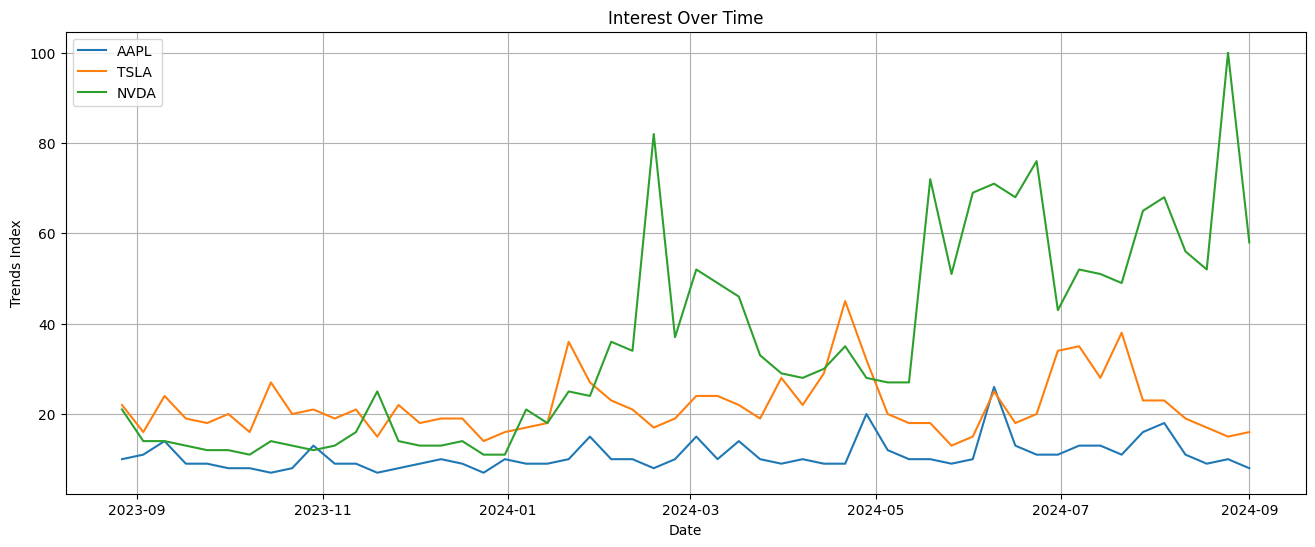
\includegraphics[width=\linewidth,height=0.6\textheight,keepaspectratio]{gfx/m4l2_notes_fig1_google_trends_aapl_tsla_nvda.png}
\par\smallskip{\small \textbf{Hình 1.1:} Mức độ quan tâm theo thời gian (Interest Over Time) trên Google Trends đối với AAPL, TSLA và NVDA, giai đoạn 2023-09-01 đến 2024-09-01}
\end{figure}

Bây giờ khi đã có biểu đồ, dưới đây là một số điểm chính cần chú ý và phân tích:

\textbf{Xu hướng tổng thể:}
\begin{itemize}
  \item Tăng/Giảm: Các xu hướng nhìn chung đang tăng, giảm hay giữ ổn định trong năm? Điều này có thể cho thấy mức độ quan tâm đối với các công ty đang tăng lên hay suy giảm.
  \item Tính mùa vụ: Ta có nhận thấy các mẫu hình hay đỉnh lặp lại vào những thời điểm nhất định trong năm không? Điều này có thể liên quan đến các đợt ra mắt sản phẩm, báo cáo tài chính hoặc các sự kiện khác.
\end{itemize}

\textbf{Mức độ phổ biến tương đối:}
\begin{itemize}
  \item So sánh: Từ khóa nào cho thấy mức độ quan tâm tổng thể cao nhất? Từ khóa nào thấp nhất? Điều này có thể cho ta ý niệm về mức độ phổ biến tương đối của các công ty này xét theo khối lượng tìm kiếm.
  \item Điểm giao nhau: Có những điểm nào mà xu hướng của các từ khóa khác nhau cắt nhau không? Điều này có thể báo hiệu sự thay đổi trong sự chú ý hoặc nhận thức của công chúng.
\end{itemize}

\textbf{Độ biến động:}
\begin{itemize}
  \item Dao động: Các xu hướng dao động nhiều đến mức nào theo thời gian? Những biến động lớn có thể cho thấy sự nhạy cảm với tin tức hoặc các sự kiện thị trường.
  \item Giá trị ngoại lai: Có đỉnh hoặc đáy đáng kể nào nổi bật không? Hãy thử tìm hiểu điều gì có thể đã gây ra chúng (ví dụ: thông báo tin tức, ra mắt sản phẩm, các vụ tranh cãi).
\end{itemize}

\textbf{Tương quan:}
\begin{itemize}
  \item Mối quan hệ: Xu hướng của các từ khóa khác nhau có vẻ di chuyển cùng nhau hay độc lập? Điều này có thể cho biết chúng có chịu ảnh hưởng của các yếu tố tương tự hay không.
\end{itemize}

Bằng cách xem xét cẩn thận các khía cạnh này của biểu đồ, chúng ta có thể có được hiểu biết về hành vi tìm kiếm liên quan đến các công ty này và có khả năng rút ra kết luận về nhận thức của công chúng cũng như hiệu quả hoạt động trên thị trường của họ.

Cụ thể với ví dụ của chúng ta, có thể quan sát thấy các đỉnh và đáy, trong đó NVIDIA (NVDA) có một đỉnh đáng kể vào khoảng tháng 3 năm 2024, gần đạt chỉ số xu hướng (trend index) là 80, và một lần nữa trong giai đoạn gần đây nhất vào cuối tháng 8 năm 2024. Chỉ số cao như vậy có thể trùng với các sự kiện quan trọng liên quan đến NVIDIA, chẳng hạn ra mắt sản phẩm, báo cáo thu nhập hoặc các diễn biến thị trường. Thực tế, vào tháng 3 năm 2024, NVIDIA đã đưa ra những thông báo quan trọng liên quan đến kiến trúc GPU thế hệ tiếp theo có tên Blackwell. Kiến trúc này có 208 tỷ bóng bán dẫn (transistor) đầy ấn tượng và được thiết kế để chạy các mô hình AI tạo sinh theo thời gian thực. Sự kỳ vọng xoay quanh Blackwell nhiều khả năng đã góp phần làm tăng mức độ quan tâm đối với NVIDIA vào thời điểm đó. Ngoài ra, vào tháng 8 năm 2024, NVIDIA tiếp tục công bố các đổi mới liên quan đến AI và hiệu năng trung tâm dữ liệu tại hội nghị Hot Chips, càng thúc đẩy mức độ quan tâm đối với công ty. Những sự kiện và tiến bộ công nghệ này nhiều khả năng giải thích các đỉnh quan tâm được quan sát đối với NVIDIA trong những tháng đó.

Apple (AAPL) và Tesla (TSLA) thể hiện các xu hướng khác nhau trong cùng giai đoạn. Trong khi cả hai công ty nhìn chung duy trì được mức quan tâm, các dao động của họ ít rõ rệt hơn so với NVIDIA. Việc phân tích tin tức hoặc các thông báo của công ty trong những khung thời gian này có thể làm sáng tỏ nguyên nhân đằng sau các xu hướng đó.

Chúng ta cũng cần cân nhắc khám phá tương quan giữa các xu hướng quan tâm đối với các công ty này và các chỉ số thị trường rộng hơn (ví dụ: S\&P 500). Nếu có tương quan dương mạnh, điều đó có thể cho thấy cảm xúc thị trường chung ảnh hưởng đến mức độ quan tâm đối với từng cổ phiếu cụ thể.

Chúng ta cũng cần quan sát bất kỳ mẫu hình lặp lại nào qua các tháng hoặc quý khác nhau. Các yếu tố mùa vụ (ví dụ: mùa lễ, mùa báo cáo thu nhập) có thể tác động đến cảm xúc của nhà đầu tư và mức độ quan tâm.

\begin{itemize}
  \item Các đỉnh của TSLA: Tesla (TSLA) thường có các đỉnh đáng chú ý vào khoảng tháng 4 và tháng 7 mỗi năm. Những đỉnh này có thể trùng với các báo cáo thu nhập hàng quý hoặc các thông báo quan trọng liên quan đến sản phẩm hoặc diễn biến kinh doanh của Tesla.
  \item Xu hướng của AAPL: Apple (AAPL) thường cho thấy xu hướng tăng đều vào khoảng tháng 9 và tháng 1. Những tháng này thường trùng với các đợt ra mắt sản phẩm mới (ví dụ: các đợt phát hành iPhone) và mùa lễ.
  \item Các dao động của NVDA: NVIDIA (NVDA) thể hiện các mẫu hình khó dự đoán hơn, nhưng có các dao động vào khoảng tháng 3 và tháng 8. Hãy tìm hiểu xem có các sự kiện hoặc hội nghị đặc thù của ngành diễn ra trong những tháng này hay không.
\end{itemize}

\subsection*{1.3 Phân tích Mức độ Quan tâm theo các Thước đo khác}

Google Trends cũng cho phép lấy các chi tiết khác liên quan đến truy vấn tìm kiếm của chúng ta:

\begin{itemize}
  \item \textbf{Mức độ quan tâm theo tiểu vùng (Interest by subregion)} cho phép ta xem mức độ quan tâm đối với một từ khóa tìm kiếm cụ thể biến thiên như thế nào giữa các khu vực địa lý khác nhau trong một vùng lớn hơn.
  \item \textbf{Các chủ đề liên quan (Related topics)} là những chủ đề hoặc khái niệm rộng hơn gắn với từ khóa của chúng ta, và cũng được những người dùng khác tìm kiếm.
  \item \textbf{Các truy vấn liên quan (Related queries)} là những từ khóa tìm kiếm cụ thể mà người ta đã dùng kết hợp với từ khóa của chúng ta. Đây là các truy vấn thực tế do những người dùng khác nhập vào công cụ tìm kiếm trong cùng khoảng thời gian.
\end{itemize}

\subsubsection*{Phân tích Mức độ Quan tâm theo Khu vực}

Bây giờ, hãy lấy mức độ quan tâm theo khu vực đối với từ khóa tìm kiếm NVDA và xác định 10 khu vực có mức độ quan tâm cao nhất:

\begin{lstlisting}[language=Python,escapeinside={(*@}{@*)}]
# (*@Khởi@*) (*@tạo@*) (*@một@*) (*@đối@*) (*@tượng@*) (*@của@*) (*@lớp@*) (*@TrendReq@*) (*@và@*) (*@xây@*) (*@dựng@*) (*@payload@*)
pytrends = TrendReq(hl='en-US', tz=360)
pytrends.build_payload(["NVDA"], timeframe='2023-09-01 2024-09-01')

# (*@Lấy@*) (*@dữ@*) (*@liệu@*) (*@mức@*) (*@độ@*) (*@quan@*) (*@tâm@*) (*@theo@*) (*@khu@*) (*@vực@*)
interest_by_region_df = pytrends.interest_by_region()
interest_by_region_df.sort_values(by='NVDA', ascending=False).head(10)
\end{lstlisting}

\begin{lstlisting}[escapeinside={(*@}{@*)}]
               NVDA
geoName
Hong Kong       100
Israel           81
Taiwan           81
United States    65
Singapore        61
Canada           57
China            33
Switzerland      16
South Korea      13
New Zealand      11
\end{lstlisting}

Kết quả này cho thấy 10 khu vực có mức độ quan tâm tìm kiếm cao nhất đối với ``NVDA'' trong giai đoạn đã chỉ định ('2023-09-01 2024-09-01'). Các giá trị biểu thị mức độ phổ biến tương đối của từ khóa tìm kiếm tại mỗi khu vực, trong đó 100 là giá trị cao nhất.

Ví dụ, Hong Kong có mức độ quan tâm tìm kiếm cao nhất đối với ``NVDA'' với giá trị 100, tiếp theo là Đài Loan và Israel với giá trị 79 mỗi nơi. [chưa rõ trong nguyên bản: kết quả chạy hiển thị Israel và Taiwan cùng bằng 81, không phải 79]

Dữ liệu này có thể hữu ích cho các doanh nghiệp để hiểu sự phân bố địa lý của mức độ quan tâm đối với sản phẩm hoặc dịch vụ của họ. Nó cũng có thể được dùng cho nghiên cứu thị trường và để nhận diện các thị trường mục tiêu tiềm năng. Xin lưu ý rằng cần phân tích thêm và đối chiếu với các nguồn dữ liệu khác để rút ra kết luận chắc chắn.

\subsubsection*{Các Truy vấn và Chủ đề Liên quan}

Các chủ đề và truy vấn liên quan hàng đầu (top) và đang tăng (rising) có thể cực kỳ hữu ích cho các tác vụ kỹ thuật tài chính vì chúng cung cấp hiểu biết về ``tâm trí tập thể của thị trường'' và bộc lộ các xu hướng có thể không hiển nhiên từ dữ liệu tài chính truyền thống.

\textbf{Các Chủ đề Liên quan (Related Topics)} là những chủ đề rộng hơn gắn với NVDA. Điều này có thể giúp nhận diện:
\begin{itemize}
  \item Xu hướng ngành: Có các xu hướng rộng hơn trong lĩnh vực game, AI hoặc trung tâm dữ liệu đang ảnh hưởng đến mức độ quan tâm đối với NVDA không?
  \item Chủ đề đầu tư: Có các chủ đề đầu tư cụ thể (ví dụ: cổ phiếu tăng trưởng, cổ phiếu công nghệ) đang thúc đẩy mức độ quan tâm đối với NVDA không?
\end{itemize}

\textbf{Các Truy vấn Liên quan (Related Queries)} là những cụm từ khác mà người ta tìm kiếm kết hợp với từ khóa NVDA. Điều này có thể cho thấy:
\begin{itemize}
  \item Xu hướng mới nổi: Có các từ khóa mới hoặc đang tăng cho thấy sự thay đổi trong mức độ quan tâm hoặc các lĩnh vực trọng tâm mới của NVDA không?
  \item Phân tích đối thủ cạnh tranh: Người ta có tìm kiếm NVDA trong sự so sánh với các đối thủ cạnh tranh của nó không?
  \item Nhận thức của công chúng: Những mối quan ngại hoặc mối quan tâm chính của mọi người về NVDA là gì?
\end{itemize}

Cả Các Chủ đề Liên quan và Các Truy vấn Liên quan đều có thể được lọc để lấy các thuật ngữ Hàng đầu (Top) và Đang tăng (Rising) cho mỗi loại:

\begin{itemize}
  \item \textbf{Top} - đây là các chủ đề/truy vấn tìm kiếm phổ biến nhất. Việc chấm điểm theo thang tương đối, trong đó 100 là chủ đề/truy vấn được tìm kiếm phổ biến nhất, 50 là truy vấn được tìm kiếm với tần suất bằng một nửa, và tiếp tục như vậy.
  \item \textbf{Rising} - đây là các chủ đề/truy vấn có mức tăng tần suất tìm kiếm lớn nhất kể từ giai đoạn trước. Các kết quả được đánh dấu ``Breakout'' có mức tăng rất lớn, có lẽ vì các chủ đề/truy vấn này là mới và có rất ít (nếu có) lượt tìm kiếm trước đó.
\end{itemize}

Trong bài học này, chúng ta sẽ tập trung vào Các Truy vấn Liên quan. Cả các truy vấn liên quan hàng đầu và đang tăng đều mang lại những hiểu biết giá trị, nhưng chúng phục vụ các mục đích khác nhau. Lựa chọn tốt nhất phụ thuộc vào các mục tiêu cụ thể và loại phân tích mà chúng ta đang thực hiện. Từ góc độ kỹ thuật tài chính, việc chọn giữa các truy vấn liên quan hàng đầu và đang tăng vẫn phụ thuộc vào mục tiêu cụ thể của chúng ta, nhưng dưới đây là một khuyến nghị được điều chỉnh sát hơn:

\begin{itemize}
  \item \textbf{Đối với Giao dịch Thuật toán và Phân tích Cảm xúc:} Các truy vấn đang tăng (rising) nhìn chung có giá trị hơn. Chúng có thể cung cấp các tín hiệu thời gian thực cho các chiến lược giao dịch dựa trên cảm xúc. Chúng ta có thể xây dựng một hệ thống tự động điều chỉnh các vị thế danh mục hoặc tạo tín hiệu giao dịch dựa trên những thay đổi trong cảm xúc được thể hiện qua các truy vấn đang tăng. Ví dụ, nếu ta quan sát thấy cảm xúc tiêu cực tăng vọt đột ngột liên quan đến một công ty mà ta đang nắm giữ trong danh mục, thuật toán có thể tự động giảm mức độ phơi nhiễm đối với cổ phiếu đó.

  \item \textbf{Đối với Quản trị Rủi ro:} Các truy vấn đang tăng có vai trò then chốt đối với các dấu hiệu cảnh báo sớm. Một đợt tăng vọt các lượt tìm kiếm cho các từ khóa liên quan đến kiện tụng, điều tra của cơ quan quản lý hoặc thu hồi sản phẩm có thể cho thấy các rủi ro tiềm ẩn đối với một công ty hoặc ngành. Chúng ta có thể tích hợp việc phân tích các truy vấn đang tăng vào hệ thống quản trị rủi ro để chủ động nhận diện và đánh giá các mối đe dọa tiềm ẩn.

  \item \textbf{Đối với Tối ưu hóa Danh mục và Phân bổ Tài sản:} Cả truy vấn hàng đầu và đang tăng đều có thể hữu ích.
  \begin{itemize}
    \item Truy vấn hàng đầu (Top): Có thể giúp hiểu các chủ đề và động lực chính của các tài sản hoặc ngành khác nhau, từ đó cho phép đa dạng hóa danh mục tương ứng.
    \item Truy vấn đang tăng (Rising): Có thể giúp nhận diện các chủ đề mới nổi hoặc các rủi ro tiềm ẩn có thể đòi hỏi điều chỉnh danh mục.
  \end{itemize}

  \item \textbf{Đối với Nghiên cứu Định lượng và Xây dựng Mô hình:} Cả hai loại truy vấn đều có thể có giá trị như các nguồn dữ liệu thay thế.
  \begin{itemize}
    \item Truy vấn đang tăng (Rising): Có thể được dùng để tạo các chỉ báo cảm xúc hoặc tín hiệu phát hiện sự kiện để đưa vào các mô hình định lượng.
    \item Truy vấn hàng đầu (Top): Có thể được dùng để hiểu mối quan hệ giữa các tài sản hoặc ngành khác nhau dựa trên các chủ đề và mối quan ngại được thể hiện trong các truy vấn tìm kiếm.
  \end{itemize}
\end{itemize}

Nhìn chung, trong khi cả hai đều có công dụng riêng, các truy vấn đang tăng có xu hướng có giá trị hơn đối với các ứng dụng kỹ thuật tài chính đòi hỏi hiểu biết theo thời gian thực và tập trung vào các xu hướng ngắn hạn cùng các thay đổi cảm xúc. Các truy vấn hàng đầu mang lại hiểu biết rộng hơn về nhận thức của thị trường, vốn có thể hữu ích cho các chiến lược dài hạn hơn và phân tích cơ bản. Hãy nhớ cân nhắc các thách thức về nhiễu, chất lượng dữ liệu, và nhu cầu về các kỹ thuật phân tích tinh vi khi làm việc với cả hai loại truy vấn.

Cũng xin lưu ý rằng việc thu hẹp khoảng thời gian khi lấy các hiểu biết từ các truy vấn liên quan đang tăng có thể rất có lợi, đặc biệt khi mục tiêu của chúng ta là phát hiện các xu hướng ngắn hạn hoặc nắm bắt các phản ứng tức thời của thị trường. Khung thời gian ngắn hơn nhìn chung mang lại sự cân bằng tốt giữa độ nhạy, khả năng có sẵn của dữ liệu và tính khả thi để hành động. Chúng ta có thể thử nghiệm với các khung thời gian khác nhau để tìm ra khung phù hợp nhất với nhu cầu cụ thể và độ biến động của các tài sản mà ta đang phân tích.

Trong Python, chúng ta có thể lấy các truy vấn liên quan hàng đầu và đang tăng cho một từ khóa tìm kiếm và phân tích kết quả:

\begin{lstlisting}[language=Python,escapeinside={(*@}{@*)}]
# (*@Khởi@*) (*@tạo@*) (*@một@*) (*@đối@*) (*@tượng@*) (*@của@*) (*@lớp@*) (*@TrendReq@*) (*@và@*) (*@xây@*) (*@dựng@*) (*@payload@*)
pytrends = TrendReq(hl='en-US', tz=360)
pytrends.build_payload(["NVDA"], timeframe='2024-08-18 2024-09-01')

# (*@Chờ@*) (*@10@*) (*@giây@*) (*@trước@*) (*@khi@*) (*@gửi@*) (*@yêu@*) (*@cầu@*) (*@tiếp@*) (*@theo@*) (*@để@*) (*@tránh@*) (*@làm@*) (*@quá@*) (*@tải@*) (*@máy@*) (*@chủ@*)
time.sleep(10)

# (*@Lấy@*) (*@các@*) (*@truy@*) (*@vấn@*) (*@liên@*) (*@quan@*)
related_queries_dict = pytrends.related_queries()

# (*@In@*) (*@các@*) (*@truy@*) (*@vấn@*) (*@liên@*) (*@quan@*) (*@hàng@*) (*@đầu@*)
print("Top related queries:")
print(related_queries_dict["NVDA"]["top"])

# (*@In@*) (*@các@*) (*@truy@*) (*@vấn@*) (*@liên@*) (*@quan@*) (*@đang@*) (*@tăng@*)
print("\nRising related queries:")
print(related_queries_dict["NVDA"]["rising"])
\end{lstlisting}

Các truy vấn đang tăng đối với ``NVDA'' cung cấp một số hiểu biết thú vị, đặc biệt liên quan đến thông báo thu nhập sắp tới. Chúng ta có thể rút ra những điều sau:

\begin{itemize}
  \item Thu nhập chiếm ưu thế: Trọng tâm áp đảo là thu nhập của NVDA. Các thuật ngữ liên quan đến thu nhập đều đang tăng mạnh mức độ quan tâm tìm kiếm. Điều này cho thấy mức độ kỳ vọng và quan tâm cao đối với kết quả tài chính của công ty.

  \item Thông tin thời gian thực: Xu hướng ``Breakout'' của ``nvda earnings time today'' cho thấy mọi người đang tích cực tìm kiếm thông tin thời gian thực về thông báo thu nhập, có thể vào ngày công bố.

  \item Mức độ quan tâm toàn cầu: Sự xuất hiện của các ký tự tiếng Nhật và tiếng Trung cho thấy mức độ quan tâm đối với thu nhập của NVDA vượt ra ngoài các khu vực nói tiếng Anh, làm nổi bật tầm với toàn cầu của công ty.

  \item Trọng tâm của nhà đầu tư: Các thuật ngữ như ``nvda investor relations'' và ``when does nvda report earnings'' cho thấy các nhà đầu tư đang tích cực tìm kiếm thông tin về việc công bố thu nhập và có thể đang chuẩn bị cho các phản ứng thị trường tiềm năng.

  \item Tài chính và Nasdaq: Sự gia tăng của ``nasdaq nvda financials'' cho thấy mọi người đang tìm kiếm thông tin tài chính chi tiết về NVDA, có thể trên trang web Nasdaq hoặc các nền tảng tài chính khác.

  \item Các cổ phiếu khác và nhiễu tiềm ẩn: Trong khi các thuật ngữ liên quan đến thu nhập chiếm ưu thế, có một số giá trị ngoại lai như ``lunr stock'', ``pdd stock'', ``crm stock'', ``chwy stock'' và ``afrm stock''. Chúng có thể liên quan đến các công ty hoặc xu hướng thị trường khác và có khả năng là nhiễu trong bối cảnh phân tích NVDA. Cần điều tra thêm để hiểu mức độ liên quan của chúng.
\end{itemize}

\subsection*{1.4 Các Lưu ý và Hạn chế khi sử dụng dữ liệu Google Trends}

Khi sử dụng dữ liệu Google Trends cho phân tích tài chính, chúng ta cần nhận thức được các hạn chế của nó. Dù dữ liệu Google Trends có thể mang lại nhiều hiểu biết, điều quan trọng là phải hiểu các hạn chế của nó về chất lượng dữ liệu. Dưới đây là một số khía cạnh chính cần ghi nhớ:

\begin{itemize}
  \item \textbf{Lấy mẫu:} Dữ liệu Google Trends dựa trên một mẫu các lượt tìm kiếm, không phải toàn bộ khối lượng tìm kiếm, và phương pháp lấy mẫu chính xác không được công bố công khai. Điều này có nghĩa là tồn tại sai số lấy mẫu vốn có, và dữ liệu có thể không đại diện hoàn hảo cho toàn bộ tổng thể các lượt tìm kiếm. Điều này cũng có nghĩa là có thể có một số nhiễu và dữ liệu có thể không phản ánh hoàn hảo mức độ quan tâm tìm kiếm thực tế.
  \item \textbf{Cập nhật dữ liệu:} Dữ liệu Google Trends có thể được cập nhật hoặc điều chỉnh theo thời gian khi Google cải tiến các thuật toán và kỹ thuật xử lý dữ liệu của mình. Điều này có nghĩa là dữ liệu lịch sử mà bạn đã truy cập trước đây có thể thay đổi đôi chút trong tương lai.
  \item \textbf{Chuẩn hóa:} Dữ liệu Google Trends được chuẩn hóa, nghĩa là các giá trị mang tính tương đối so với điểm cao nhất trong khung thời gian bạn chọn. Dữ liệu được chuẩn hóa về thang từ 0 đến 100. Giá trị 100 biểu thị mức phổ biến đỉnh điểm, trong khi các giá trị khác được co giãn theo tỷ lệ. Điều này có nghĩa là các giá trị biểu thị mức độ phổ biến tương đối của một từ khóa tìm kiếm so với điểm cao nhất trong khung thời gian được chọn. Trong khi việc chuẩn hóa giúp so sánh các xu hướng, nó cũng có thể che khuất khối lượng tìm kiếm tuyệt đối, vốn có thể liên quan trong một số trường hợp.
  \item \textbf{Độ chi tiết địa lý:} Mức độ chi tiết về địa lý của dữ liệu Google Trends thay đổi tùy theo từ khóa tìm kiếm và khoảng thời gian. Với một số từ khóa hoặc khu vực, dữ liệu có thể chi tiết hơn, trong khi với những nơi khác, dữ liệu có thể mang tính tổng hợp hơn. Điều này có thể ảnh hưởng đến độ chính xác của phân tích theo khu vực.
  \item \textbf{Các yếu tố bên ngoài:} Hành vi tìm kiếm có thể chịu ảnh hưởng của nhiều yếu tố bên ngoài, như mức độ đưa tin của truyền thông, các sự kiện tin tức, tính mùa vụ, và thậm chí mức độ phổ biến của các từ khóa tìm kiếm khác. Những yếu tố này có thể đưa nhiễu và thiên lệch vào dữ liệu, gây khó khăn cho việc tách biệt các xu hướng nền tảng thực sự.
  \item \textbf{Quyền riêng tư:} Dữ liệu Google Trends đã được ẩn danh hóa và tổng hợp, nhưng vẫn cần lưu ý đến các cân nhắc về quyền riêng tư, đặc biệt khi xử lý các chủ đề nhạy cảm.
\end{itemize}

Bằng cách hiểu các cân nhắc về chất lượng dữ liệu này và thực hiện các biện pháp phòng ngừa phù hợp, chúng ta có thể sử dụng dữ liệu Google Trends hiệu quả hơn và rút ra các kết luận đáng tin cậy hơn cho phân tích tài chính. Hãy nhớ rằng bối cảnh là chìa khóa. Chúng ta cần xem xét bối cảnh xung quanh dữ liệu, chẳng hạn các yếu tố bên ngoài tiềm năng có thể đang ảnh hưởng đến hành vi tìm kiếm.

\section*{2. Phân tích Ngữ nghĩa Tiềm ẩn (Latent Semantic Analysis)}

Cho đến nay chúng ta đã khám phá dữ liệu Google Trends và các ví dụ đơn giản về việc dùng \texttt{pytrends} để thu thập dữ liệu. Trong khi bản thân \texttt{pytrends} cung cấp những hiểu biết giá trị về các xu hướng tìm kiếm, việc đưa vào các kỹ thuật học máy như Phân tích Ngữ nghĩa Tiềm ẩn (LSA) có thể mang lại nhiều lợi thế.

Trước khi giới thiệu LSA, chúng ta cần hiểu một số thuật ngữ. Trong ngữ cảnh của LSA, một ``\textbf{tài liệu}'' (document) là một đơn vị văn bản mà chúng ta muốn phân tích. Nó có thể là bất cứ thứ gì từ một câu đơn lẻ đến cả một bài báo, một cuốn sách, hoặc thậm chí một tập hợp các văn bản liên quan. Điều then chốt là nó đại diện cho một phần thông tin riêng biệt mà chúng ta muốn so sánh và phân tích trong mối quan hệ với các tài liệu khác. Dưới đây là một số ví dụ về những gì có thể được coi là một ``tài liệu'' trong các ứng dụng LSA khác nhau:

\begin{itemize}
  \item \textbf{Mô hình hóa chủ đề (Topic Modeling):} Mỗi tài liệu có thể là một bài báo, một bài blog, hoặc một bài đăng trên mạng xã hội. LSA có thể giúp nhận diện các chủ đề chính được thảo luận trong các tài liệu này.
  \item \textbf{Truy xuất thông tin (Information Retrieval):} Mỗi tài liệu có thể là một trang web, một bài nghiên cứu, hoặc một mô tả sản phẩm. LSA có thể giúp tìm các tài liệu tương tự về mặt ngữ nghĩa với một truy vấn cho trước.
  \item \textbf{Phân loại tài liệu (Document Classification):} Mỗi tài liệu có thể là một email, một đánh giá của khách hàng, hoặc một hợp đồng pháp lý. LSA có thể giúp phân loại các tài liệu này dựa trên nội dung của chúng.
\end{itemize}

Phân tích Ngữ nghĩa Tiềm ẩn (LSA) là một kỹ thuật trong xử lý ngôn ngữ tự nhiên, phân tích mối quan hệ giữa một tập hợp các tài liệu và các thuật ngữ mà chúng chứa bằng cách tạo ra một tập hợp các khái niệm liên quan đến các tài liệu và thuật ngữ. LSA giả định rằng những từ có nghĩa gần nhau sẽ xuất hiện trong các đoạn văn bản tương tự. Việc đưa vào các kỹ thuật học máy như LSA có thể mang lại nhiều lợi thế:

\begin{itemize}
  \item \textbf{Khám phá các mối quan hệ ẩn:} LSA có thể bộc lộ các mối quan hệ ẩn giữa các thuật ngữ và khái niệm mà có thể không hiển nhiên khi chỉ nhìn vào dữ liệu tìm kiếm thô. Điều này có thể giúp ta hiểu cấu trúc ngữ nghĩa nền tảng của các truy vấn tìm kiếm liên quan đến các tài liệu của chúng ta.

  \item \textbf{Giảm chiều dữ liệu:} LSA có thể giảm số chiều của dữ liệu bằng cách biểu diễn nó trong một không gian khái niệm có số chiều thấp hơn. Điều này có thể giúp phân tích và trực quan hóa dữ liệu dễ dàng hơn, đặc biệt khi xử lý số lượng lớn thuật ngữ.

  \item \textbf{Cải thiện tìm kiếm và gợi ý:} Bằng cách hiểu mối quan hệ giữa các thuật ngữ và khái niệm, chúng ta có thể xây dựng các công cụ tìm kiếm và hệ thống gợi ý thông minh hơn. Ví dụ, ta có thể gợi ý các tìm kiếm liên quan hoặc đề xuất tài liệu dựa trên độ tương đồng ngữ nghĩa thay vì chỉ khớp từ khóa.

  \item \textbf{Mô hình hóa chủ đề:} LSA có thể được dùng cho mô hình hóa chủ đề, cho phép ta khám phá các chủ đề hoặc đề tài chính hiện diện trong một tập hợp tài liệu hoặc truy vấn tìm kiếm. Điều này có thể giúp ta hiểu bối cảnh rộng hơn của thông tin và có khả năng phân loại hoặc phân cụm tài liệu hiệu quả hơn.
\end{itemize}

Nói ngắn gọn, LSA được dùng để phân tích dữ liệu văn bản và là một phương pháp trích xuất và biểu diễn ý nghĩa theo cách dùng trong ngữ cảnh của các từ, thông qua các tính toán thống kê áp dụng trên một kho ngữ liệu văn bản lớn. LSA là một công cụ mạnh để phân tích dữ liệu văn bản, nhưng có một số hạn chế. Ví dụ, nó không xử lý tốt hiện tượng đa nghĩa (polysemy, các từ có nhiều nghĩa) hay đồng nghĩa (synonymy, các từ khác nhau có cùng nghĩa).

Trong bài học này, chúng ta sẽ khám phá một ví dụ cơ bản về cách có thể dùng LSA để phân tích các từ khóa tìm kiếm liên quan và cải thiện hiểu biết của chúng ta về hành vi tìm kiếm của người dùng. Việc coi cái gì là một tài liệu phụ thuộc vào ứng dụng cụ thể và loại phân tích mà ta muốn thực hiện. Điều quan trọng là đảm bảo các tài liệu của chúng ta có ý nghĩa và phù hợp với tác vụ đang thực hiện. Một tập hợp các tài liệu được gọi chung là ``\textbf{ma trận thuật ngữ-tài liệu}'' (term-document matrix).

Các kỹ sư tài chính có thể tiếp cận việc hình thành tài liệu cho LSA hoặc các kỹ thuật tương tự theo những cách khác nhau:

\begin{itemize}
  \item Chuyên môn lĩnh vực: Các kỹ sư tài chính thường có chuyên môn sâu về lĩnh vực và cẩn thận chọn các từ khóa và cụm từ dựa trên hiểu biết của họ về thị trường tài chính, các tài sản cụ thể và các sự kiện liên quan.

  \item Nguồn dữ liệu: Họ có thể sử dụng phạm vi nguồn dữ liệu rộng hơn so với chỉ Google Trends, chẳng hạn các bài báo tin tức và phân tích cảm xúc, dữ liệu mạng xã hội, hồ sơ công ty và bản ghi các cuộc họp báo cáo thu nhập, các tập dữ liệu độc quyền.

  \item Tiền xử lý tinh vi: Họ có thể sử dụng các kỹ thuật xử lý ngôn ngữ tự nhiên nâng cao hơn cho bước tiền xử lý, bao gồm nhận dạng thực thể có tên (nhận diện các công ty, con người, địa điểm), phân tích cảm xúc (gán điểm cảm xúc cho văn bản), mô hình hóa chủ đề (nhận diện các chủ đề nền tảng trong tài liệu).

  \item Các phương pháp tổ hợp (Ensemble Methods): Họ có thể kết hợp LSA với các kỹ thuật học máy khác hoặc dùng các phương pháp tổ hợp để cải thiện độ chính xác và tính vững của mô hình.

  \item Kiểm định lùi và xác thực (Backtesting and Validation): Các kỹ sư tài chính kiểm định lùi và xác thực các mô hình của họ một cách nghiêm ngặt bằng dữ liệu lịch sử để đảm bảo chúng đáng tin cậy và có khả năng tạo ra các tín hiệu giao dịch hoặc chiến lược đầu tư sinh lời.
\end{itemize}

Với ví dụ của chúng ta, chúng ta sẽ tạo ma trận thuật ngữ-tài liệu với tập hợp các tài liệu sau:

\begin{quote}
Document 1: ``Risk management in derivatives trading'', \\
Document 2: ``Portfolio optimization techniques and strategies'', \\
Document 3: ``Algorithmic trading and its impact on market efficiency'', \\
Document 4: ``Quantitative methods for financial modeling'', \\
Document 5: ``High-frequency trading and liquidity provision'', \\
Document 6: ``Integrating Derivatives into Portfolio Optimization Strategies'', \\
Document 7: ``High-Frequency Trading Strategies: Algorithmic Approaches and Market Impact'', \\
Document 8: ``Quantitative Methods for Algorithmic Trading and Portfolio Optimization''
\end{quote}

Trước khi tiếp tục với mã, hãy lưu ý rằng các tài liệu trong ma trận thuật ngữ-tài liệu của chúng ta chứa những từ như ``in'', ``and'', ``for'', ``on''. Những từ này được gọi là \textbf{từ dừng} (stop words). Chúng là các từ thông dụng, nhìn chung không mang nhiều ý nghĩa cụ thể trong ngữ cảnh phân tích văn bản. Thường có lợi khi loại bỏ từ dừng khỏi dữ liệu văn bản trước khi tạo ma trận thuật ngữ-tài liệu. Điều này có thể giúp:

\begin{itemize}
  \item \textbf{Giảm nhiễu:} Từ dừng có thể thêm nhiễu vào dữ liệu và che khuất các thuật ngữ quan trọng hơn vốn truyền tải các chủ đề hoặc đề tài chính.
  \item \textbf{Cải thiện hiệu quả:} Loại bỏ từ dừng có thể giảm kích thước ma trận, giúp việc tính toán nhanh và hiệu quả hơn.
  \item \textbf{Tập trung vào các thuật ngữ liên quan:} Bằng cách loại bỏ các từ thông dụng, chúng ta có thể tập trung vào các thuật ngữ có ý nghĩa hơn, đặc thù cho các tài liệu và ứng dụng của mình.
\end{itemize}

Chúng ta cũng sẽ áp dụng kỹ thuật lemmatization (chuẩn hóa về dạng gốc từ điển). \textbf{Stemming (rút gọn về gốc từ) và lemmatization} là hai kỹ thuật tiền xử lý văn bản được dùng trong Xử lý ngôn ngữ tự nhiên (NLP) giúp rút gọn các từ về dạng cơ sở của chúng.
\begin{itemize}
  \item \textbf{Stemming} rút gọn các từ về thân từ (stem), vốn không nhất thiết là từ có thật, bằng cách loại bỏ tiền tố và hậu tố. Ví dụ ``playing'' sẽ thành ``play'', ``studies'' sẽ thành ``studi'', và ``happily'' sẽ thành ``happi''.
  \item \textbf{Lemmatization} rút gọn các từ về dạng từ điển hoặc dạng cơ sở gọi là lemma. Ví dụ ``playing'' sẽ thành ``play'', ``studies'' sẽ thành ``study'', và ``better'' sẽ thành ``good''.
\end{itemize}

Trong ví dụ của chúng ta, chúng ta sử dụng lemmatization: với ngôn ngữ đặc thù và có thể có nhiều sắc thái của tài chính, lemmatization nhiều khả năng có lợi hơn stemming. Nó có thể giúp nhóm các dạng khác nhau của từ (ví dụ: ``analyze'', ``analyzing'', ``analysis'') trong khi vẫn giữ được ý nghĩa cốt lõi của chúng.

Bây giờ khi đã làm rõ mọi thuật ngữ cơ bản và định nghĩa LSA, hãy tiến hành chuẩn bị dữ liệu. Đoạn mã Python sau thực hiện đúng việc đó:

\begin{lstlisting}[language=Python,escapeinside={(*@}{@*)}]
# (*@Các@*) (*@tài@*) (*@liệu@*) (*@mẫu@*)
documents = [
    "Risk management in derivatives trading",
    "Portfolio optimization techniques and strategies",
    "Algorithmic trading and its impact on market efficiency",
    "Quantitative methods for financial modeling",
    "High-frequency trading and liquidity provision",
    "Integrating Derivatives into Portfolio Optimization Strategies",
    "High-Frequency Trading Strategies: Algorithmic Approaches and Market Impact",
    "Quantitative Methods for Algorithmic Trading and Portfolio Optimization"
]

# (*@Tải@*) (*@stopwords@*) (*@và@*) (*@tài@*) (*@nguyên@*) (*@WordNet@*) (*@rồi@*) (*@tạo@*) (*@một@*) (*@đối@*) (*@tượng@*) (*@Lemmatizer@*)
nltk.download('stopwords')
nltk.download('wordnet')
nltk.download('punkt')
lemmatizer = WordNetLemmatizer()

# (*@Xây@*) (*@dựng@*) (*@hàm@*) (*@tiền@*) (*@xử@*) (*@lý@*) (*@văn@*) (*@bản@*)
def preprocess_text(text):
    text = re.sub(r'[^\w\s-]', '', text)  # (*@Loại@*) (*@bỏ@*) (*@dấu@*) (*@câu@*) (*@ngoại@*) (*@trừ@*) (*@dấu@*) (*@gạch@*) (*@nối@*)
    tokens = nltk.word_tokenize(text.lower())
    tokens = [lemmatizer.lemmatize(token) for token in tokens] # (*@Lemmatize@*)
    stop_words = set(stopwords.words('english')) # (*@định@*) (*@nghĩa@*) (*@stop\_words@*) (*@là@*) (*@tập@*) (*@hợp@*) (*@các@*) (*@từ@*) (*@dừng@*) (*@tiếng@*) (*@Anh@*)
    tokens = [token for token in tokens if token not in stop_words] # (*@Loại@*) (*@bỏ@*) (*@từ@*) (*@dừng@*)
    return tokens

# (*@Tạo@*) (*@một@*) (*@đối@*) (*@tượng@*) (*@CountVectorizer@*)
vectorizer = CountVectorizer(tokenizer=preprocess_text, token_pattern=None)

# (*@Tạo@*) (*@ma@*) (*@trận@*) (*@thuật@*) (*@ngữ-tài@*) (*@liệu,@*) (*@rồi@*) (*@chuyển@*) (*@thành@*) (*@một@*) (*@DataFrame@*) (*@của@*) (*@pandas@*)
term_document_matrix = vectorizer.fit_transform(documents)
df = pd.DataFrame(term_document_matrix.toarray(), columns = vectorizer.get_feature_names_out())
term_document_matrix = df.T
print(term_document_matrix)
\end{lstlisting}

Ma trận này cho thấy các mối quan hệ giữa các thuật ngữ (hàng) và các tài liệu (cột). Ví dụ:

\begin{itemize}
  \item Thuật ngữ ``algorithmic'' xuất hiện (giá trị 1) trong các tài liệu 3, 7 và 8.
  \item Thuật ngữ ``trading'' xuất hiện trong các tài liệu 1, 3, 5, 7 và 8.
  \item Tài liệu 1 chứa các thuật ngữ ``derivatives'', ``management'', ``risk'' và ``trading''.
\end{itemize}

Ma trận này là nền tảng để áp dụng LSA hoặc các kỹ thuật giảm chiều khác.

\subsection*{2.1 LSA liên hệ với SVD như thế nào}

LSA sử dụng Phân rã Giá trị Kỳ dị (Singular Value Decomposition, SVD) ở cốt lõi để tìm các mối quan hệ ẩn giữa các thuật ngữ và khái niệm. Phân rã Giá trị Kỳ dị là một khái niệm nền tảng trong đại số tuyến tính và là một kỹ thuật mạnh được dùng trong nhiều lĩnh vực, bao gồm học máy và xử lý ngôn ngữ tự nhiên. Cách thức hoạt động như sau:

\begin{enumerate}
  \item Ma trận Tài liệu-Thuật ngữ: LSA bắt đầu với một ma trận tài liệu-thuật ngữ, trong đó mỗi hàng đại diện cho một tài liệu và mỗi cột đại diện cho một thuật ngữ (từ). Các ô chứa tần suất của mỗi thuật ngữ trong mỗi tài liệu.

  \item Áp dụng SVD hay Phân tích Ma trận thành nhân tử: SVD được áp dụng lên ma trận Tài liệu-Thuật ngữ. SVD là một cách phân tích (chia nhỏ) một ma trận thành ba ma trận riêng biệt. Nó phân rã ma trận thành ba ma trận:
  \begin{itemize}
    \item $U$: Biểu diễn độ tương đồng giữa tài liệu và khái niệm.
    \item $\Sigma$: Một ma trận đường chéo chứa các giá trị kỳ dị, biểu diễn tầm quan trọng của mỗi khái niệm.
    \item $V$: Biểu diễn độ tương đồng giữa thuật ngữ và khái niệm.
    \item Công thức: Mối quan hệ giữa ma trận gốc ($A$) và các ma trận phân rã là: $A = U \Sigma V^T$ (trong đó $V^T$ là chuyển vị của $V$).
  \end{itemize}

  \item Giảm chiều: Bằng cách chỉ giữ lại các giá trị kỳ dị lớn nhất (và các cột/hàng tương ứng trong $U$ và $V$), chúng ta giảm số chiều (khái niệm) trong khi vẫn bảo toàn thông tin quan trọng nhất. Điều này tương tự Phân tích Thành phần Chính (PCA).

  \item Không gian Khái niệm: Các ma trận thu được biểu diễn các tài liệu và thuật ngữ trong một ``không gian khái niệm'' mới. Các từ có nghĩa tương tự sẽ nằm gần nhau hơn trong không gian này, ngay cả khi chúng không xuất hiện trong cùng các tài liệu.
\end{enumerate}

Về bản chất, SVD trong LSA giúp:

\begin{itemize}
  \item \textbf{Khám phá các mối quan hệ tiềm ẩn:} Nhận diện các khái niệm nền tảng không hiện diện tường minh trong văn bản.
  \item \textbf{Giảm nhiễu:} Lọc bỏ thông tin ít quan trọng hơn và tập trung vào ý nghĩa cốt lõi.
  \item \textbf{Cải thiện truy xuất thông tin:} Biểu diễn tài liệu và truy vấn theo cách nắm bắt được độ tương đồng ngữ nghĩa.
\end{itemize}

Quá trình này cho phép LSA vượt ra ngoài việc khớp từ khóa đơn giản và hiểu ý nghĩa của văn bản ở mức sâu hơn.

Bây giờ hãy tiếp tục với mã Python, trong đó chúng ta sẽ dùng \texttt{TruncatedSVD} từ \texttt{scikit-learn}, về bản chất là thực hiện Phân rã Giá trị Kỳ dị (SVD) ở bên dưới. \texttt{TruncatedSVD} là một cách triển khai SVD hiệu quả được thiết kế riêng cho việc giảm chiều. Nó tính SVD rồi chỉ giữ lại \texttt{n\_components} giá trị kỳ dị lớn nhất cùng các vector tương ứng của chúng. Phiên bản SVD rút gọn (truncated) này là thứ tạo ra \texttt{lsa\_matrix}, biểu diễn dữ liệu của chúng ta trong một không gian khái niệm có số chiều thấp hơn.

\textbf{Quan trọng:} Kết quả đầu ra của LSA có thể khác nhau mỗi lần chúng ta chạy mã. Điều này là do việc khởi tạo ngẫu nhiên của thuật toán \texttt{TruncatedSVD}. Sự biến thiên liên quan đến bản chất của Phân rã Giá trị Kỳ dị (SVD) và cách LSA sử dụng nó. Dưới đây là phân tích các yếu tố chính:

\begin{itemize}
  \item Phép quay trong Không gian Khái niệm: SVD về bản chất tìm cách tốt nhất để biểu diễn dữ liệu của chúng ta trong một ``không gian khái niệm'' mới. Các thành phần (hay chiều) trong không gian này được xác định bằng cách tìm các hướng có phương sai lớn nhất trong dữ liệu gốc. Tuy nhiên, thường có một mức độ linh hoạt trong cách các thành phần này được định hướng (xoay). Hãy hình dung như việc xoay một vật thể 3D: vật thể vẫn như cũ, nhưng phép chiếu của nó lên các trục thay đổi.

  \item Tính mơ hồ về dấu: Dấu (dương hoặc âm) của các giá trị trong kết quả LSA có thể đảo mà không làm thay đổi ý nghĩa nền tảng. Đó là vì hướng của một thành phần là tùy ý. Hãy tưởng tượng một thành phần biểu diễn ``financial modeling'': việc nó hướng về một phía hay phía ngược lại không quan trọng, nó vẫn nắm bắt cùng một khái niệm.

  \item Độ nhạy với các thay đổi nhỏ: SVD có thể nhạy cảm với các thay đổi nhỏ trong dữ liệu đầu vào. Ngay cả những biến thể nhỏ về tần suất từ hoặc việc thêm/bớt một vài tài liệu cũng có thể dẫn đến một mức độ xoay nào đó trong không gian khái niệm, dẫn đến các trọng số thuật ngữ (term loadings) khác nhau.

  \item Khởi tạo ngẫu nhiên: Như đã đề cập, thuật toán TruncatedSVD thường dùng khởi tạo ngẫu nhiên, điều này có thể góp phần gây ra các biến thể trong kết quả.
\end{itemize}

Trong khi những biến thể này có vẻ đáng lo ngại, chúng thường không làm thay đổi đáng kể cách diễn giải tổng thể các kết quả LSA. Vị trí tương đối của các thuật ngữ trong không gian khái niệm và các mẫu hình tương đồng chung nhìn chung được bảo toàn. Để đảm bảo kết quả nhất quán, chúng ta sẽ đặt tham số \texttt{random\_state} về một giá trị cố định khi tạo đối tượng \texttt{TruncatedSVD}. Điều này sẽ cho ra cùng một kết quả mỗi lần chúng ta chạy mã.

\begin{lstlisting}[language=Python,escapeinside={(*@}{@*)}]
# (*@Lấy@*) (*@các@*) (*@thuật@*) (*@ngữ@*) (*@(từ)@*) (*@từ@*) (*@ma@*) (*@trận@*) (*@thuật@*) (*@ngữ-tài@*) (*@liệu@*)
terms = term_document_matrix.index

# (*@Tạo@*) (*@một@*) (*@mô@*) (*@hình@*) (*@LSA@*) (*@và@*) (*@khớp@*) (*@với@*) (*@term\_document\_matrix@*)
lsa = TruncatedSVD(n_components=2, random_state=42)
lsa_matrix = lsa.fit_transform(term_document_matrix)

# (*@Tạo@*) (*@DataFrame@*) (*@cho@*) (*@kết@*) (*@quả@*) (*@LSA@*) (*@với@*) (*@tên@*) (*@thuật@*) (*@ngữ@*) (*@và@*) (*@in@*) (*@ra@*)
df_lsa = pd.DataFrame(lsa_matrix, index=terms)
print(df_lsa)
\end{lstlisting}

Việc diễn giải các kết quả LSA đòi hỏi hiểu không gian ngữ nghĩa mới được tạo ra bởi việc giảm chiều và phân tích các mối quan hệ giữa thuật ngữ và tài liệu trong không gian này. Dưới đây là cách diễn giải các kết quả:

\begin{itemize}
  \item Diễn giải các cột: Chúng còn được gọi là Thành phần (Components) hay Khái niệm (Concepts) hay Chiều (Dimensions). Hãy coi mỗi thành phần như đại diện cho một ``khái niệm'' hoặc ``chủ đề'' ẩn trong các tài liệu.
  \item Diễn giải các hàng: Mỗi hàng trong ma trận này đại diện cho một thuật ngữ từ ma trận gốc của chúng ta, nhưng nay được chiếu lên một không gian khái niệm 2 chiều (vì chúng ta chọn \texttt{n\_components=2}).
  \item Diễn giải các giá trị:
  \begin{itemize}
    \item Hai giá trị trong mỗi hàng biểu diễn tọa độ của thuật ngữ đó trong không gian khái niệm mới. Các thuật ngữ có tọa độ tương tự nằm gần nhau hơn trong không gian khái niệm, cho thấy mối quan hệ ngữ nghĩa. Trong ví dụ của chúng ta, hàng đầu tiên đại diện cho thuật ngữ ``algorithmic''. Tọa độ của nó xấp xỉ (1.488 -0.458). Nếu một thuật ngữ khác có tọa độ tương tự, điều đó cho thấy các thuật ngữ này có liên quan trong ngữ cảnh các tài liệu của chúng ta.
    \item Các giá trị biểu diễn trọng số (loading) của thuật ngữ đó trên thành phần tương ứng. Các trọng số cho ta biết mỗi thuật ngữ đóng góp bao nhiêu vào khái niệm đó. Ví dụ, ``algorithmic'' và ``trading'' có trọng số cao trên Thành phần 1, cho thấy Thành phần 1 đại diện cho khái niệm ``algorithmic trading''. Giá trị càng cao (dương hoặc âm) cho thấy mối liên hệ giữa thuật ngữ và thành phần đó càng mạnh.
  \end{itemize}
\end{itemize}

Từ kết quả đầu ra của mã, chúng ta có thể diễn giải mối quan hệ giữa các thuật ngữ bằng cách xem xét tọa độ của chúng và rút ra một số quan sát sơ bộ:

\begin{itemize}
  \item \textbf{Các cụm riêng biệt:}
  \begin{itemize}
    \item Cụm Giao dịch (Trading): ``algorithmic'', ``high-frequency'', ``impact'', ``market'' và ``trading'' có giá trị cao ở thành phần 0 và chủ yếu là giá trị âm ở thành phần 1. Điều này củng cố ý tưởng rằng thành phần 0 đại diện cho các khái niệm liên quan đến giao dịch tự động và tần suất cao, cùng tác động tiềm ẩn của chúng lên thị trường.

    \item Cụm Danh mục đầu tư và Tối ưu hóa: ``optimization'' và ``portfolio'' tạo thành một cụm rõ ràng với giá trị dương cao ở cả hai thành phần. Điều này cho thấy mối liên hệ mạnh giữa các thuật ngữ này, có khả năng liên quan đến các kỹ thuật tối ưu hóa danh mục đầu tư.

    \item Cụm Phái sinh và Phương pháp-Định lượng: Việc nhóm ``method'', ``quantitative'' và ``derivative'' lại với nhau cho thấy một mối liên hệ tiềm năng giữa các phương pháp định lượng và ứng dụng của chúng vào các công cụ phái sinh.

    \item Cụm Quản lý-Rủi ro-Thanh khoản-Cung ứng: Việc kết hợp ``management'', ``risk'', ``liquidity'' và ``provision'' cho thấy một cụm liên quan đến việc quản lý rủi ro tài chính và đảm bảo thanh khoản. Điều này cũng có vẻ hợp lý, vì các khái niệm này thường đan xen trong các bối cảnh tài chính, đặc biệt khi xử lý các công cụ phái sinh hoặc hoạt động giao dịch.
  \end{itemize}

  \item \textbf{Các quan sát khác:}
  \begin{itemize}
    \item ``Trading'' như một khái niệm trung tâm: ``trading'' có giá trị cao nhất ở thành phần 0, cho thấy tầm quan trọng của nó và mối liên hệ tiềm năng với nhiều hình thức giao dịch được thảo luận trong các tài liệu.
    \item Cặp riêng biệt: Cặp thuật ngữ ``financial'' và ``modeling'' tạo thành một cặp rất riêng biệt do có tọa độ giống hệt nhau. Cần phân tích thêm để xác định mối quan hệ của chúng với các thuật ngữ và cụm khác.
    \item Sự chồng lấn giữa các cụm: Một số thuật ngữ, như ``strategy'' và ``technique'', có giá trị vừa phải ở nhiều thành phần, cho thấy khả năng chồng lấn hoặc kết nối giữa các cụm khác nhau.
  \end{itemize}
\end{itemize}

Phân tích nhanh này cho một cái nhìn tổng quan khá tốt về mối quan hệ giữa các thuật ngữ dựa trên kết quả LSA.

Bây giờ chúng ta có thể vẽ các tọa độ để trực quan hóa chúng và xác nhận xem các cụm được đề xuất này có xuất hiện gần nhau trong biểu diễn trực quan hay không. Để thực hiện điều này, chúng ta sẽ dùng mô-đun \texttt{plotly.graph\_objects} được nhập với tên \texttt{go}:

\begin{lstlisting}[language=Python,escapeinside={(*@}{@*)}]
# (*@Tạo@*) (*@danh@*) (*@sách@*) (*@các@*) (*@văn@*) (*@bản@*) (*@hiển@*) (*@thị@*) (*@khi@*) (*@rê@*) (*@chuột@*) (*@(hover)@*) (*@với@*) (*@nhãn@*) (*@và@*) (*@tọa@*) (*@độ@*)
hover_texts = []
for row in df_lsa.values:
    terms = df_lsa.index[(df_lsa[0] == row[0]) & (df_lsa[1] == row[1])]
    terms_str = ', '.join([f'"{term}"' for term in terms])
    coord = f"({row[0]:.5f}, {row[1]:.5f})"
    hover_texts.append(f"Terms: {terms_str}<br>{coord}")

# (*@Tạo@*) (*@biểu@*) (*@đồ@*) (*@phân@*) (*@tán@*)
fig = go.Figure(go.Scatter(
    x=df_lsa[0],
    y=df_lsa[1],
    mode='markers',
    marker=go.scatter.Marker(
        size=10,
        color='blue',
        opacity=0.8
    ),
    hovertemplate='%{text}<extra></extra>',
    text=hover_texts
))

# (*@Đặt@*) (*@nhãn@*) (*@trục@*) (*@và@*) (*@tiêu@*) (*@đề@*)
fig.update_layout(
    xaxis_title="Component 0",
    yaxis_title="Component 1",
    title="LSA Results Scatter Plot"
)

fig.show()
\end{lstlisting}

Các biểu đồ Plotly có tính tương tác theo mặc định. Chúng ta có thể dùng các tính năng tương tác của nó để kéo/thu phóng và rê chuột/chọn để xem chú giải công cụ (tooltip) với nhãn thuật ngữ và tọa độ.

Bây giờ nhìn vào biểu đồ này, có vẻ như các cụm không dễ trực quan hóa lắm. Có vẻ chúng ta đã quá tập trung vào các giá trị vừa phải của tọa độ thuật ngữ, mà không chú ý đủ đến khoảng cách chính xác giữa chúng. Để xác định các cụm chính xác hơn, chúng ta nên dùng các phương pháp hình thức hơn. Bằng cách sử dụng các phương pháp này, chúng ta có thể tránh các diễn giải chủ quan và xác định các cụm chính xác hơn dựa trên các thước đo định lượng về độ tương đồng hoặc khoảng cách. Chúng ta sẽ xem xét các phương pháp này ở phần sau của bài học.

\subsection*{2.2 Những Cân nhắc Quan trọng với LSA và SVD}

\subsubsection*{Chọn số thành phần tối ưu cho LSA}

Việc chọn số thành phần tối ưu (\texttt{n\_components}) cho LSA là một bước then chốt. Dưới đây là một số cân nhắc:

\begin{itemize}
  \item \textbf{Bắt đầu nhỏ:} Bắt đầu với số lượng thành phần nhỏ (ví dụ: 2, 3 hoặc 5) để xem liệu nó có cho hiểu biết ban đầu tốt về mối quan hệ giữa thuật ngữ và tài liệu hay không. Điều này có thể giúp nắm bắt cảm nhận về dữ liệu và nhận diện các cụm hoặc chủ đề tiềm năng.
  \item \textbf{Tăng dần lặp lại:} Tăng dần số lượng thành phần và quan sát cách diễn giải các kết quả thay đổi. Hãy tìm điểm mà việc thêm thành phần không còn cải thiện đáng kể khả năng diễn giải hoặc không bộc lộ thêm các mối quan hệ có ý nghĩa mới.
  \item \textbf{Cân nhắc kích thước kho ngữ liệu:} Với các kho ngữ liệu nhỏ hơn, ít thành phần hơn có thể là đủ để tránh quá khớp (overfitting). Với các kho ngữ liệu lớn hơn, nhiều thành phần hơn có thể nắm bắt các mối quan hệ ngữ nghĩa tinh tế hơn.
  \item \textbf{Tập trung vào sự mạch lạc ngữ nghĩa:} Đánh giá sự mạch lạc ngữ nghĩa của các chủ đề hoặc cụm thu được. Các thuật ngữ trong mỗi cụm có hợp lý khi đi cùng nhau không? Các cụm có riêng biệt và có ý nghĩa không? Nếu độ mạch lạc giảm khi ta thêm thành phần, đó có thể là dấu hiệu cho thấy ta bắt đầu quá khớp.
  \item \textbf{Cân bằng giữa giảm chiều và mất thông tin:} LSA liên quan đến sự đánh đổi giữa giảm số chiều và bảo toàn thông tin. Chúng ta nên tìm điểm cân bằng tối ưu, nơi ta có số lượng thành phần có thể quản lý được trong khi vẫn nắm bắt các mối quan hệ ngữ nghĩa quan trọng nhất.
\end{itemize}

Tóm lại, không có câu trả lời chung cho mọi trường hợp về số thành phần tối ưu trong LSA. Nó phụ thuộc vào dữ liệu và mục tiêu cụ thể. Chúng ta cần thử nghiệm với các giá trị khác nhau, đánh giá cẩn thận các kết quả, và dùng kiến thức lĩnh vực để định hướng lựa chọn.

\subsubsection*{Hiểu các hạn chế của LSA và SVD}

Như quan sát từ ví dụ trên, một số thuật ngữ được gom cụm vì chúng xuất hiện trong một tài liệu cụ thể. Ví dụ ``algorithmic'', ``high-frequency'', ``impact'', ``market'' và ``trading'' là các thuật ngữ tương tự tạo thành một cụm. Và tất cả chúng đều đến từ tài liệu 7.

Đây là một điểm then chốt về Phân tích Ngữ nghĩa Tiềm ẩn (LSA) và các hạn chế tiềm ẩn của nó. Nếu LSA liên tục gom cụm các thuật ngữ chỉ dựa trên sự đồng xuất hiện của chúng trong cùng một tài liệu, điều đó đặt ra câu hỏi về hiệu quả của nó trong việc nắm bắt các mối quan hệ ngữ nghĩa rộng hơn.

Dưới đây là phân tích lý do điều này có thể xảy ra và ý nghĩa của nó đối với LSA:

\begin{itemize}
  \item \textbf{Ngữ cảnh đặc thù của tài liệu:} LSA chủ yếu dựa vào các mẫu hình đồng xuất hiện của từ trong một kho ngữ liệu. Nếu các thuật ngữ thường xuyên xuất hiện cùng nhau trong một tài liệu đơn lẻ nhưng không xuất hiện trên toàn bộ kho ngữ liệu, LSA có thể diễn giải chúng là có liên quan về ngữ nghĩa ngay cả khi ý nghĩa ngữ cảnh rộng hơn của chúng khác nhau đáng kể.
  \item \textbf{Kích thước hoặc tính đa dạng hạn chế của kho ngữ liệu:} Một kho ngữ liệu nhỏ hoặc đồng nhất có thể làm trầm trọng thêm vấn đề này. Nếu các tài liệu trong kho ngữ liệu thiếu đa dạng về chủ đề và cách dùng ngôn ngữ, LSA có thể gặp khó khăn trong việc nhận diện các mối quan hệ ngữ nghĩa rộng hơn ngoài sự đồng xuất hiện ở cấp độ tài liệu.
  \item \textbf{Tính thưa của dữ liệu:} Trong LSA, ma trận thuật ngữ-tài liệu có thể rất thưa, đặc biệt với từ vựng lớn. Tính thưa này đôi khi có thể khiến mô hình tập trung vào các mẫu hình đồng xuất hiện cục bộ trong tài liệu thay vì các mối quan hệ ngữ nghĩa toàn cục.
\end{itemize}

Vậy, LSA có ích gì nếu nó chủ yếu nhận diện các cụm ở cấp độ tài liệu? Dù kịch bản chúng ta gặp phải không lý tưởng, LSA vẫn có thể mang lại những hiểu biết giá trị:

\begin{itemize}
  \item \textbf{Tóm tắt tài liệu:} LSA có thể hiệu quả trong việc nhận diện các thuật ngữ và khái niệm chính trong từng tài liệu riêng lẻ, hữu ích cho việc tóm tắt và trích xuất chủ đề.
  \item \textbf{Giảm chiều dữ liệu:} Ngay cả khi các cụm mang tính đặc thù theo tài liệu, LSA vẫn giảm số chiều của dữ liệu hiệu quả, giúp việc phân tích và trực quan hóa dễ dàng hơn.
  \item \textbf{Nền tảng cho các kỹ thuật khác:} LSA có thể đóng vai trò nền tảng cho các kỹ thuật mô hình hóa chủ đề nâng cao hơn giải quyết các hạn chế của nó, chẳng hạn Latent Dirichlet Allocation (LDA).
\end{itemize}

Để cải thiện hiệu suất của LSA và nắm bắt các mối quan hệ ngữ nghĩa rộng hơn:

\begin{itemize}
  \item \textbf{Tăng kích thước và tính đa dạng của kho ngữ liệu:} Đưa vào phạm vi tài liệu rộng hơn về các chủ đề khác nhau với cách dùng ngôn ngữ đa dạng.
  \item \textbf{Tiền xử lý và Kỹ thuật đặc trưng:} Tiền xử lý văn bản cẩn thận (ví dụ: loại bỏ từ dừng, stemming/lemmatization) và cân nhắc dùng các sơ đồ trọng số khác nhau (ví dụ: Tần suất Thuật ngữ-Nghịch đảo Tần suất Tài liệu, viết tắt là TF-IDF, một thống kê số học được dùng trong truy xuất thông tin và khai phá văn bản để phản ánh mức độ quan trọng của một từ đối với một tài liệu trong một bộ sưu tập hay kho ngữ liệu) nhằm nhấn mạnh các thuật ngữ giàu thông tin hơn.
  \item \textbf{Khám phá các kỹ thuật khác:} Cân nhắc dùng các kỹ thuật mô hình hóa chủ đề thay thế như LDA, vốn mô hình hóa tường minh phân phối của các chủ đề trong tài liệu.
\end{itemize}

Tóm lại, trong khi LSA có thể hữu ích cho phân tích ở cấp độ tài liệu, cần xem xét các hạn chế của nó trong việc nắm bắt các mối quan hệ ngữ nghĩa rộng hơn. Đảm bảo một kho ngữ liệu đa dạng và mang tính đại diện, cùng việc khám phá các kỹ thuật thay thế, có thể giúp vượt qua các hạn chế này và phát huy toàn bộ tiềm năng của mô hình hóa chủ đề.

\section*{3. Tính các Thước đo Độ tương đồng}

Trong tiểu mục này, chúng ta sẽ áp dụng một số thước đo độ tương đồng lên các kết quả LSA của mình để phân tích thêm các thuật ngữ trong không gian LSA.

Nhìn chung, không nên chỉ dựa vào một thước đo độ tương đồng duy nhất, đặc biệt khi khám phá các tập dữ liệu hoặc tác vụ phức tạp. Các thước đo độ tương đồng khác nhau có điểm mạnh và điểm yếu khác nhau và có thể nắm bắt các khía cạnh khác nhau của độ tương đồng.

\subsection*{3.1 Thước đo độ tương đồng cosine giữa các thuật ngữ}

Độ tương đồng cosine là một cách phổ biến để đo độ tương đồng giữa các vector trong không gian LSA. Đoạn mã sau giúp lượng hóa độ tương đồng ngữ nghĩa giữa các thuật ngữ trong cụm riêng biệt đầu tiên (các thuật ngữ: ``algorithmic'', ``high-frequency'', ``impact'', ``market'', ``trading'') dựa trên biểu diễn của chúng trong không gian khái niệm LSA:

\begin{lstlisting}[language=Python,escapeinside={(*@}{@*)}]
# (*@Trích@*) (*@xuất@*) (*@các@*) (*@vector@*) (*@thuật@*) (*@ngữ@*) (*@cho@*) (*@cụm@*) (*@riêng@*) (*@biệt@*) (*@đầu@*) (*@tiên@*)
terms_cl1 = ["algorithmic", "high-frequency", "impact", "market", "trading"]
term_vectors_cl1 = df_lsa.loc[terms_cl1]

# (*@Tính@*) (*@độ@*) (*@tương@*) (*@đồng@*) (*@cosine@*)
similarity_matrix = cosine_similarity(term_vectors_cl1)

# (*@Chuyển@*) (*@thành@*) (*@DataFrame@*) (*@để@*) (*@trực@*) (*@quan@*) (*@hóa@*) (*@tốt@*) (*@hơn@*)
similarity_df = pd.DataFrame(similarity_matrix, index=terms_cl1, columns=terms_cl1)

# (*@In@*) (*@kết@*) (*@quả@*) (*@cho@*) (*@cụm@*) (*@riêng@*) (*@biệt@*) (*@đầu@*) (*@tiên@*) (*@kèm@*) (*@nhãn@*)
print("Cosine similarity for first distinct cluster:")
print(similarity_df)
\end{lstlisting}

Ma trận này cho thấy độ tương đồng cosine theo từng cặp giữa các thuật ngữ trong cụm riêng biệt đầu tiên. Các giá trị nằm trong khoảng từ 0 đến 1, trong đó 1 biểu thị độ tương đồng hoàn hảo và 0 biểu thị không có độ tương đồng. Dưới đây là một số quan sát:

\begin{itemize}
  \item Độ tương đồng cao trong cụm: Hầu hết các giá trị trong ma trận gần 1, cho thấy các thuật ngữ trong cụm này có độ tương đồng ngữ nghĩa cao. Điều này là dự kiến vì chúng đã được nhận diện là một cụm trong phân tích LSA.
  \item ``Impact'' và ``market'' tương đồng hoàn hảo: Độ tương đồng cosine giữa ``impact'' và ``market'' là 1, cho thấy chúng được coi là đồng nghĩa trong ngữ cảnh của kho ngữ liệu này.
  \item ``Algorithmic'' và ``trading'' rất tương đồng: Độ tương đồng cosine giữa ``algorithmic'' và ``trading'' rất cao (0.998), cho thấy mối liên hệ ngữ nghĩa mạnh giữa các thuật ngữ này. Điều này hợp lý vì ``algorithmic trading'' là một khái niệm phổ biến.
  \item ``High-frequency'' kém tương đồng hơn đôi chút: ``High-frequency'' có điểm tương đồng thấp hơn một chút so với các thuật ngữ khác, cho thấy nó có thể có ý nghĩa hoặc ngữ cảnh hơi khác trong cụm này.
\end{itemize}

Phân tích này xác nhận rằng các thuật ngữ trong cụm riêng biệt đầu tiên quả thực có liên quan về mặt ngữ nghĩa dựa trên độ tương đồng cosine của chúng.

Bây giờ hãy tính độ tương đồng cosine cho các thuật ngữ trong cụm thứ tư:

\begin{lstlisting}[language=Python,escapeinside={(*@}{@*)}]
# (*@Trích@*) (*@xuất@*) (*@các@*) (*@vector@*) (*@thuật@*) (*@ngữ@*) (*@cho@*) (*@cụm@*) (*@thứ@*) (*@tư@*)
terms_cl4 = ["management", "risk", "liquidity", "provision"]
term_vectors_cl4 = df_lsa.loc[terms_cl4]

# (*@Tính@*) (*@độ@*) (*@tương@*) (*@đồng@*) (*@cosine@*)
similarity_matrix = cosine_similarity(term_vectors_cl4)

# (*@Chuyển@*) (*@thành@*) (*@DataFrame@*) (*@để@*) (*@trực@*) (*@quan@*) (*@hóa@*) (*@tốt@*) (*@hơn@*)
similarity_df = pd.DataFrame(similarity_matrix, index=terms_cl4, columns=terms_cl4)

# (*@In@*) (*@kết@*) (*@quả@*) (*@cho@*) (*@cụm@*) (*@thứ@*) (*@tư@*) (*@kèm@*) (*@nhãn@*)
print("Cosine similarity for fourth cluster:")
print(similarity_df)
\end{lstlisting}

Ở đây chúng ta có:

\begin{itemize}
  \item Độ tương đồng hoàn hảo: ``Management'' và ``risk'' có độ tương đồng cosine bằng 1, cho thấy chúng được coi là có liên quan rất chặt chẽ hoặc thậm chí đồng nghĩa trong ngữ cảnh này. Tương tự, ``liquidity'' và ``provision'' cũng cho thấy độ tương đồng hoàn hảo. Điều này không đáng ngạc nhiên vì độ tương đồng cosine đo góc giữa hai vector. Vì ``Management'' và ``risk'' có tọa độ giống hệt nhau, chúng hướng về cùng một phía, dẫn đến góc 0 độ và độ tương đồng cosine bằng 1. Tương tự, ``liquidity'' và ``provision'' cũng tạo thành một cặp vector giống hệt nhau khác.

  \item Độ tương đồng mạnh nhưng chưa hoàn hảo: Trong khi các thuật ngữ khác thể hiện độ tương đồng mạnh, nó không hoàn hảo (độ tương đồng cosine là 0.82). Điều này cho thấy có mức độ chồng lấn ngữ nghĩa nhưng cũng có một số khác biệt trong ý nghĩa của chúng trong các tài liệu.
\end{itemize}

Cụm này cho thấy rõ trọng tâm là quản lý rủi ro, có khả năng làm nổi bật tầm quan trọng của việc cung ứng thanh khoản trong việc giảm thiểu các rủi ro tài chính.

Chúng ta có thể tiếp tục cách tiếp cận này bằng cách chọn các cụm cụ thể và phân tích độ tương đồng cosine trong các nhóm đó. Điều này cho phép ta tập trung vào các thuật ngữ đã biết là có liên quan và khám phá các mối liên hệ ngữ nghĩa chi tiết hơn.

Bằng cách sử dụng cách tiếp cận có mục tiêu hơn, chúng ta có thể thu được những hiểu biết có ý nghĩa hơn từ phân tích độ tương đồng cosine và hiểu rõ hơn cấu trúc ngữ nghĩa của dữ liệu.

Một cách để khám phá mối quan hệ giữa các cụm là tính tâm (centroid) của mỗi cụm rồi đo độ tương đồng cosine giữa các tâm. Điều này có thể giúp ta hiểu các chủ đề hoặc khái niệm khác nhau liên hệ với nhau như thế nào.

Trước đó chúng ta đã nhận diện bốn cụm riêng biệt và một cặp riêng biệt: cặp thuật ngữ ``financial'' và ``modeling''. Hãy phân tích thêm cặp này để xác định mối quan hệ của nó với các thuật ngữ và cụm khác.

\begin{lstlisting}[language=Python,escapeinside={(*@}{@*)}]
# (*@Trích@*) (*@xuất@*) (*@các@*) (*@vector@*) (*@thuật@*) (*@ngữ@*) (*@cho@*) (*@cặp@*) (*@riêng@*) (*@biệt@*)
terms_pair = ["financial", "modeling"]
term_vectors_pair = df_lsa.loc[terms_pair]

# (*@Trích@*) (*@xuất@*) (*@các@*) (*@vector@*) (*@thuật@*) (*@ngữ@*) (*@cho@*) (*@cụm@*) (*@thứ@*) (*@hai@*) (*@và@*) (*@thứ@*) (*@ba@*)
term_vectors_cl2 = df_lsa.loc[["optimization", "portfolio"]]
term_vectors_cl3 = df_lsa.loc[["derivative", "method", "quantitative"]]


# (*@Tính@*) (*@tâm@*) (*@cho@*) (*@cặp@*) (*@riêng@*) (*@biệt@*)
centroid_pair = term_vectors_pair.mean()

# (*@Lưu@*) (*@các@*) (*@vector@*) (*@thuật@*) (*@ngữ@*) (*@của@*) (*@các@*) (*@cụm@*) (*@vào@*) (*@một@*) (*@danh@*) (*@sách@*) (*@và@*) (*@tính@*) (*@tâm@*) (*@cho@*) (*@từng@*) (*@cụm@*)
cluster_term_vectors = [term_vectors_cl1, term_vectors_cl2, term_vectors_cl3, term_vectors_cl4]
centroids = [term_vectors.mean() for term_vectors in cluster_term_vectors]


# (*@Tính@*) (*@độ@*) (*@tương@*) (*@đồng@*) (*@cosine@*) (*@giữa@*) (*@cặp@*) (*@riêng@*) (*@biệt@*) (*@và@*) (*@tâm@*) (*@của@*) (*@từng@*) (*@cụm@*)
similarities = [cosine_similarity(centroid_pair.values.reshape(1, -1), centroid.values.reshape(1, -1)) for centroid in centroids]

# (*@In@*) (*@các@*) (*@độ@*) (*@tương@*) (*@đồng@*)
for i, similarity in enumerate(similarities):
  print(f"Cosine similarity between distinct pair and cluster {i+1}:", similarity)
\end{lstlisting}

Các kết quả này cho thấy độ tương đồng cosine giữa cặp riêng biệt và từng cụm trong bốn cụm. Cách diễn giải như sau:

\begin{itemize}
  \item Tương đồng mạnh nhất với cụm 2: Cặp riêng biệt có độ tương đồng cosine cao nhất (0.997) với cụm 2. Điều này cho thấy cặp này có liên hệ rất chặt chẽ với các khái niệm hoặc thuật ngữ được biểu diễn bởi cụm 2.
  \item Tương đồng vừa phải với cụm 3: Có mức tương đồng vừa phải (0.961) với cụm 3, cho thấy có một số chồng lấn về ý nghĩa hoặc ngữ cảnh.
  \item Tương đồng yếu với cụm 1 và 4: Cặp này cho thấy độ tương đồng rất yếu với cụm 1 (0.084) và 4 (0.056), cho thấy các cụm này đại diện cho các khái niệm riêng biệt không liên hệ chặt chẽ với cặp.
\end{itemize}

Kết luận: Dựa trên các kết quả này, chúng ta có thể kết luận rằng cặp riêng biệt gắn kết mạnh nhất với cụm 2, cùng một mối liên hệ vừa phải với cụm 3. Nhiều khả năng cặp này có sự chồng lấn ngữ nghĩa đáng kể với các thuật ngữ trong cụm 2.

\subsection*{3.2 Độ tương đồng cosine giữa các tài liệu}

Đo độ tương đồng cosine giữa các tài liệu hoàn chỉnh là một trong những ứng dụng phổ biến của độ tương đồng cosine trong xử lý ngôn ngữ tự nhiên và truy xuất thông tin.

Để làm điều này, trước tiên chúng ta cần lấy các \textbf{vector tài liệu} (Document vectors). Có một vài kỹ thuật để thực hiện, như lấy các vector LSA, nhúng từ (Word embeddings) và Tần suất Thuật ngữ-Nghịch đảo Tần suất Tài liệu (TF-IDF).

Trong bài học của chúng ta, chúng ta sẽ tập trung vào các vector TF-IDF vì chúng nắm bắt tầm quan trọng của các từ trong một tài liệu so với một bộ sưu tập các tài liệu. Đoạn mã sau tính độ tương đồng cosine giữa các tài liệu bằng TF-IDF và trình bày kết quả trong một dataframe.

\begin{lstlisting}[language=Python,escapeinside={(*@}{@*)}]
# (*@Tạo@*) (*@một@*) (*@đối@*) (*@tượng@*) (*@TfidfVectorizer@*) (*@và@*) (*@khớp@*) (*@với@*) (*@các@*) (*@tài@*) (*@liệu@*)
tfidf_vectorizer = TfidfVectorizer(tokenizer=preprocess_text, token_pattern=None)
tfidf_matrix = tfidf_vectorizer.fit_transform(documents)

# (*@Tính@*) (*@ma@*) (*@trận@*) (*@độ@*) (*@tương@*) (*@đồng@*) (*@cosine@*)
cosine_sim = cosine_similarity(tfidf_matrix)

# (*@Trình@*) (*@bày@*) (*@ma@*) (*@trận@*) (*@TF-IDF@*) (*@dưới@*) (*@dạng@*) (*@DataFrame@*)
short_labels = ['Doc ' + str(i+1) for i in range(len(documents))]
df = pd.DataFrame(cosine_sim, index=short_labels, columns=short_labels)
df
\end{lstlisting}

Ở đây \texttt{TfidfVectorizer} được khởi tạo với chính hàm \texttt{preprocess\_text} mà chúng ta đã dùng trước đó để tiền xử lý văn bản tài liệu trong phân tích LSA. Hàm này được truyền làm đối số cho tham số tokenizer bên trong \texttt{TfidfVectorizer}. Bằng cách dùng hàm \texttt{preprocess\_text} làm bộ tách token (tokenizer), chúng ta đảm bảo phép tính TF-IDF dựa trên các token đã được lemmatize và làm sạch, điều này có thể dẫn đến kết quả có ý nghĩa và chính xác hơn. \texttt{TfidfVectorizer} sẽ áp dụng hàm này cho từng tài liệu trong kho ngữ liệu để chuyển văn bản thô thành một chuỗi các token (từ hoặc thuật ngữ).

Cả \texttt{TfidfVectorizer} và \texttt{CountVectorizer} mà chúng ta đã dùng trước đó đều được dùng trong \texttt{scikit-learn} cho phân tích văn bản để chuyển một tập hợp các tài liệu văn bản thành một ma trận các đặc trưng số. Tuy nhiên, chúng khác nhau ở cách biểu diễn tầm quan trọng của các từ trong tài liệu:

\begin{itemize}
  \item \texttt{CountVectorizer}: Tạo một ma trận trong đó mỗi phần tử biểu diễn số lần một từ xuất hiện trong một tài liệu (tần suất thuật ngữ). Đây là một cách đơn giản để biểu diễn dữ liệu văn bản bằng số, nhưng nó không xét đến tầm quan trọng tương đối của các từ trên toàn bộ kho ngữ liệu. \texttt{CountVectorizer} tập trung vào tầm quan trọng cục bộ của các từ trong một tài liệu.

  \item \texttt{TfidfVectorizer}: Tạo một ma trận trong đó mỗi phần tử biểu diễn điểm TF-IDF của một từ trong một tài liệu. TF-IDF (Tần suất Thuật ngữ-Nghịch đảo Tần suất Tài liệu) tính đến cả tần suất của một từ trong một tài liệu và độ hiếm của nó trên toàn bộ kho ngữ liệu. Điều này có nghĩa là những từ thường xuyên xuất hiện trong một tài liệu nhưng hiếm trong kho ngữ liệu sẽ có điểm TF-IDF cao hơn, cho thấy tầm quan trọng của chúng đối với tài liệu cụ thể đó. \texttt{TfidfVectorizer} tập trung vào tầm quan trọng toàn cục của các từ so với toàn bộ kho ngữ liệu.
\end{itemize}

Bây giờ hãy phân tích kết quả đầu ra của mã. DataFrame ở trên cho thấy độ tương đồng cosine giữa các tài liệu. Dưới đây là một số quan sát dựa trên các điểm độ tương đồng cosine:

\begin{itemize}
  \item Tài liệu 6 và Tài liệu 2 tương đồng nhất (0.54). Điều này hợp lý vì cả hai tài liệu đều thảo luận về tối ưu hóa danh mục đầu tư.
  \item Tài liệu 7 và Tài liệu 3 cũng khá tương đồng (0.59), điều này là dự kiến vì cả hai đều đề cập đến giao dịch thuật toán.
  \item Tài liệu 8 có vẻ tương đồng vừa phải với nhiều tài liệu, bao gồm Tài liệu 2 (0.36), Tài liệu 6 (0.32), và Tài liệu 4 (0.42). Điều này là do nó bao quát nhiều chủ đề rộng hơn, bao gồm giao dịch thuật toán và tối ưu hóa danh mục đầu tư.
  \item Tài liệu 1 và Tài liệu 5 có độ tương đồng thấp (0.10) với hầu hết các tài liệu khác vì chúng lần lượt thảo luận về quản lý rủi ro và cung ứng thanh khoản, là những chủ đề tương đối rộng.
\end{itemize}

Dưới đây là một số hiểu biết tiềm năng mà chúng ta có thể rút ra:

\begin{itemize}
  \item Các tài liệu liên quan đến tối ưu hóa danh mục đầu tư (2 và 6) tạo thành một cụm các chủ đề liên quan.
  \item Giao dịch thuật toán (3 và 7) là một cụm khái niệm liên quan khác.
  \item Tài liệu 8 đóng vai trò cầu nối giữa hai cụm này, cho thấy có sự chồng lấn giữa các chủ đề.
  \item Quản lý rủi ro (1) và cung ứng thanh khoản (5) là các khái niệm tương đối độc lập trong tập dữ liệu này.
\end{itemize}

Xin lưu ý rằng đây chỉ là những quan sát ban đầu. Ta có thể đi sâu hơn vào chính các tài liệu để hiểu các sắc thái của độ tương đồng giữa chúng và cách các thuật ngữ cụ thể đóng góp vào các điểm độ tương đồng cosine.

Hãy nhớ rằng độ tương đồng cosine chỉ là một thước đo độ tương đồng. Tùy theo nhu cầu cụ thể và bản chất của dữ liệu, chúng ta có thể cần khám phá các thước đo độ tương đồng khác.

\subsection*{3.3 Chỉ số Jaccard}

Bây giờ hãy xem xét dùng chỉ số Jaccard làm thước đo để ước lượng độ tương đồng giữa các tài liệu của chúng ta. Trong đoạn mã sau, chúng ta xây dựng hàm \texttt{jaccard\_similarity} tính độ tương đồng Jaccard giữa hai tài liệu đã được tiền xử lý. Bên trong hàm này, chúng ta áp dụng các phương thức có sẵn \texttt{intersection} và \texttt{union} dành cho các đối tượng tập hợp (set) trong Python. Sau đó chỉ số Jaccard được tính đơn giản bằng cách chia kích thước của giao cho kích thước của hợp: \texttt{intersection / union}. Chúng ta sẽ áp dụng hàm này cho mọi cặp có thể có trong kho tài liệu của mình để tính tất cả các chỉ số theo từng cặp:

\begin{lstlisting}[language=Python,escapeinside={(*@}{@*)}]
# (*@Các@*) (*@tài@*) (*@liệu@*) (*@mẫu@*)
documents = [
    "Risk management in derivatives trading",
    "Portfolio optimization techniques and strategies",
    "Algorithmic trading and its impact on market efficiency",
    "Quantitative methods for financial modeling",
    "High-frequency trading and liquidity provision",
    "Integrating Derivatives into Portfolio Optimization Strategies",
    "High-Frequency Trading Strategies: Algorithmic Approaches and Market Impact",
    "Quantitative Methods for Algorithmic Trading and Portfolio Optimization"
]

# (*@Tải@*) (*@stopwords,@*) (*@tài@*) (*@nguyên@*) (*@WordNet@*) (*@và@*) (*@tạo@*) (*@một@*) (*@đối@*) (*@tượng@*) (*@Lemmatizer@*)
nltk.download('stopwords')
nltk.download('wordnet')
nltk.download('punkt')
lemmatizer = WordNetLemmatizer()

# (*@Hàm@*) (*@tiền@*) (*@xử@*) (*@lý@*)
def preprocess_text(text):
    text = re.sub(r'[^\w\s-]', '', text)  # (*@Loại@*) (*@bỏ@*) (*@dấu@*) (*@câu@*) (*@ngoại@*) (*@trừ@*) (*@dấu@*) (*@gạch@*) (*@nối@*)
    tokens = nltk.word_tokenize(text.lower())
    tokens = [lemmatizer.lemmatize(token) for token in tokens] # (*@Lemmatize@*)
    stop_words = set(stopwords.words('english')) # (*@định@*) (*@nghĩa@*) (*@stop\_words@*) (*@là@*) (*@tập@*) (*@hợp@*) (*@các@*) (*@từ@*) (*@dừng@*) (*@tiếng@*) (*@Anh@*)
    tokens = [token for token in tokens if token not in stop_words] # (*@Loại@*) (*@bỏ@*) (*@từ@*) (*@dừng@*)
    return tokens


# (*@Hàm@*) (*@tính@*) (*@độ@*) (*@tương@*) (*@đồng@*) (*@Jaccard@*) (*@giữa@*) (*@hai@*) (*@tài@*) (*@liệu@*)
def jaccard_similarity(doc1, doc2):
    # (*@Tiền@*) (*@xử@*) (*@lý@*) (*@các@*) (*@tài@*) (*@liệu@*)
    tokens1 = set(preprocess_text(doc1))
    tokens2 = set(preprocess_text(doc2))

    # (*@Tính@*) (*@độ@*) (*@tương@*) (*@đồng@*) (*@Jaccard@*)
    intersection = len(tokens1.intersection(tokens2))
    union = len(tokens1.union(tokens2))
    return intersection / union

# (*@Tính@*) (*@ma@*) (*@trận@*) (*@độ@*) (*@tương@*) (*@đồng@*) (*@Jaccard@*)
jaccard_sim = [[jaccard_similarity(doc1, doc2) for doc2 in documents] for doc1 in documents]

# (*@Trình@*) (*@bày@*) (*@ma@*) (*@trận@*) (*@độ@*) (*@tương@*) (*@đồng@*) (*@Jaccard@*) (*@dưới@*) (*@dạng@*) (*@DataFrame@*)
short_labels = ['Doc ' + str(i+1) for i in range(len(documents))]
df = pd.DataFrame(jaccard_sim, index=short_labels, columns=short_labels)
df
\end{lstlisting}

Ở đây chúng ta quan sát thấy:
\begin{itemize}
  \item Độ tương đồng mạnh giữa Tài liệu 2 và 6 với điểm độ tương đồng cao nhất (0.50) và cũng giữa tài liệu 3 và 7 với điểm độ tương đồng cũng là (0.50).
  \item Độ tương đồng vừa phải: Tài liệu 8 một lần nữa cho thấy độ tương đồng vừa phải với Tài liệu 2 (0.25), 4 (0.25) và 6 (0.22).
  \item Độ tương đồng thấp: Tài liệu 1 và 5 một lần nữa thể hiện độ tương đồng thấp.
\end{itemize}

So sánh với độ tương đồng Cosine: Các mẫu hình tương đồng chung tương đối nhất quán với kết quả độ tương đồng cosine. Tuy nhiên, chỉ số Jaccard có xu hướng cho điểm độ tương đồng thấp hơn nhìn chung, vì nó tập trung vào sự chồng lấn của các thuật ngữ và không xét đến tần suất thuật ngữ hay nghịch đảo tần suất tài liệu.

\section*{Kết luận}

Đến cuối bài học này, bạn nên có hiểu biết vững chắc về cách dùng Python và Google Trends để phân tích các xu hướng tìm kiếm. Bạn nên có khả năng lấy và so sánh mức độ quan tâm theo thời gian cho nhiều từ khóa tìm kiếm, phân tích mức độ quan tâm theo khu vực, và khám phá các truy vấn liên quan hàng đầu (top) và đang tăng (rising). Trong bài học này, chúng ta cũng đã khám phá cách tận dụng khoa học dữ liệu và học máy cho phân tích tài chính, với trọng tâm là phân tích các xu hướng tìm kiếm từ dữ liệu Google Trends. Bài học đã đề cập các kỹ thuật như TF-IDF và LSA để trích xuất thông tin từ văn bản, và minh họa cách thu thập và phân tích dữ liệu Google Trends bằng Python và thư viện \texttt{pytrends}. Notebook cũng đã thảo luận việc ứng dụng các kỹ thuật này cho phân tích cảm xúc, quản trị rủi ro và tối ưu hóa danh mục đầu tư.

\textbf{Tài liệu tham khảo}

\begin{itemize}
  \item Vrba, G. (2018). Timing The Market With Google Trends Search Volume Data. [online] Seeking Alpha. Available at: \url{https://seekingalpha.com/article/4202781-timing-market-google-trends-search-volume-data}.
\end{itemize}

\begin{center}
\small Copyright 2024 WorldQuant University. Nội dung này chỉ được cấp phép cho mục đích sử dụng cá nhân. Nghiêm cấm phân phối lại hoặc xuất bản tài liệu này.
\end{center}
